
\documentclass[
  reprint,            % journal-like 2-column
  amsmath,amssymb,    % math packages
  aps,pre,              % APS + Physical Review E style    
  superscriptaddress        
]{revtex4-2}

% ---- Core packages APS samples rely on ----
\usepackage{graphicx} % \inputgraphics
\usepackage{dcolumn}  % decimal-aligned tables
\usepackage{bm}       % bold math
\usepackage[T1]{fontenc}
\usepackage[utf8]{inputenc}

% Hyperlinks (APS allows it; keep unobtrusive)
\usepackage[colorlinks=true, allcolors=blue]{hyperref}


% PACKAGES FOR LANGUAGE AND FONT
\usepackage{verbatim} % For code blocks

% PACKAGES FOR ALGORITHMS (PSEUDO-CODE)
\usepackage{etoolbox} 
\usepackage{algorithm}

% PACKAGES FOR IMAGES
\usepackage{tikz} % A package for high-quality hand-made figures.
\usetikzlibrary{}
% \usepackage{float}
\usepackage[percent]{overpic} % For adding annotations to figures
% \usepackage{graphbox} 

% FOR TABLES
\usepackage{array}     % enables m{...}, >{...}, \arraybackslash, etc.
\usepackage{booktabs}  % enables \toprule \midrule \bottomrule

% STANDARD MATH PACKAGES
\usepackage{mathtools}
\usepackage{cases}
\usepackage{xfrac}

% OTHER PACKAGES
\usepackage{lipsum} % DUMMY PACKAGE

% Graphics search paths
\graphicspath{{Images/}}

% Miscellaneous operators
\DeclareMathOperator{\arctanh}{arctanh}

\newcommand{\bea}{\begin{eqnarray}} % Shortcut for equation arrays
\newcommand{\eea}{\end{eqnarray}}
\newcommand{\e}[1]{\times 10^{#1}}  % Powers of 10 notation
\def\norm#1{\|#1\|} %Norm

% Commonly used symbols
\renewcommand{\a}{\alpha}
\renewcommand{\b}{\beta}
\renewcommand{\k}{\kappa}
\newcommand{\w}{\omega}
\newcommand{\wB}{\omega_B}
\newcommand{\wZ}{\omega_0}
\newcommand{\wz}{\omega_z}
\newcommand{\wpm}{\omega_\pm}
\newcommand{\neff}{n_{eff}}
\newcommand{\dn}{\delta n}
\newcommand{\dnbar}{\overline{\delta n}_{eff}}
\newcommand{\dt}{\delta \tau}

\newcommand{\Skenderas}{Sk\"{e}nderas}

\pdfpageattr{/Rotate 0}

% =======================
% Document
% =======================
\begin{document}

\preprint{APS/123-QED} % optional

\title{Modelling and Analysis of Semiconductor Lasers Under Fiber Bragg Grating Feedback}

\author{J. Steele}
\email{jste924@aucklanduni.ac.nz}
\affiliation{Dodd--Walls Centre for Photonic and Quantum Technologies, New Zealand}
\affiliation{Department of Mathematics, University of Auckland, New Zealand}

\author{B. Krauskopf}
\affiliation{Dodd--Walls Centre for Photonic and Quantum Technologies, New Zealand}
\affiliation{Department of Mathematics, University of Auckland, New Zealand}

\author{N. Broderick}
\affiliation{Dodd--Walls Centre for Photonic and Quantum Technologies, New Zealand}
\affiliation{Department of Physics, University of Auckland, New Zealand}


\date{\today}

% ---- Abstract kept modular: put the whole environment in Sections/Abstract.tex ----

\input{Sections/0Abstract}

%\keywords{Suggested keywords}%Use showkeys class option if keyword
                              %display desired

\maketitle

% =======================
% Main text (modular)
% =======================
% Use \input so each section gets its own .aux (these will land in build/Sections/ with your latexmkrc)
% File names below are examples; create the matching files in Sections/ with no spaces in names.
% !TeX root = ../main.tex
\section{Introduction}
\label{sec:introduction}
%
Semiconductor lasers are fundamental components in modern photonic technologies.
Their emission wavelengths align with those used in optical communication networks, making them valuable light sources. 
In addition, they are orders of magnitude smaller than typical helium–neon lasers, with coherence lengths of only a few millimetres compared to many metres, which enables widespread practical applications \cite{heiskanen2018photobiomodulation}.
Semiconductor lasers are not only smaller than conventional gas lasers, but also exhibit much higher output coupling, with approximately 70\% of the light intensity escaping them compared to 1-5\% for gas lasers \cite{vantartwijk1995semiconductor}.
However, this openness makes semiconductor lasers more susceptible to external disturbances, leading to a strong response to incident signals.
Although undesirable in practical applications, this sensitivity has made semiconductor lasers a central platform for investigating nonlinear dynamics induced by external optical feedback.
The influence of external light on laser operation has been extensively investigated since the 1970s, with particular focus on conventional optical feedback (COF), typically achieved by reflecting output laser light back into the laser cavity using a mirror, as well as on optical injection of laser light from another laser \cite{weiss1991dynamics}.
Feedback and injection mechanisms have important practical implications: for example, the former arises in the operation of CD players, while the latter is central to laser amplification systems.
Beyond their direct historical significance, semiconductor lasers with feedback underpin key technologies in modern photonics. 
Feedback control is exploited to stabilize frequency and linewidth in coherent optical communication \cite{tkach2003regimes}, to enhance sensitivity in precision sensing and metrology, and to enable secure chaos-based encryption schemes \cite{uchida2008fast}. 
At the same time, semiconductor lasers with feedback provide a prototypical and experimentally accessible example of delay differential equations (DDEs), serving as a testbed for nonlinear dynamics with relevance extending to control theory \cite{stepan1989retarded}, electronics, and biological systems \cite{mackey1977oscillation}.
%
%
\subsection{Lang-Kobayashi equations}
A major breakthrough occurred in 1980 with the seminal work of Lang and Kobayashi, who introduced the Lang–Kobayashi (LK) rate equations to describe the dynamics of a semiconductor laser subject to COF from a distant external mirror \cite{lang1980external}.
The LK equations describe the time evolution of the complex electric field $E = E_x + iE_y$ and the carrier inversion $N$ under the influence of external feedback $F(t)$.
A nondimensionalized form of these equations, highlighting the key parameters governing the system dynamics, is given by \eqref{eq:LK} \cite{heil2003delay}
%
\begin{equation}
\label{eq:LK}
    \begin{aligned}
        \frac{d E}{d t} & =(1+i \a) N(t) E(t)+\eta F(t) \\
        T \frac{d N}{d t} & =P-N(t)-(1+2 N(t))|E(t)|^2
    \end{aligned}
\end{equation}
%
where $F(t) = e^{-i\wZ\tau} E(t-\tau)$. 
These key parameters can be separated into intrinsic laser parameters and external cavity (EC) parameters. 
The laser, emitting at a single frequency $\w_0$, is characterised by the pump current $P$, the linewidth enhancement factor $\a$, and the ratio of photon and electron decay times $T = \tau_e/\tau_p$. 
The EC is characterised by the round-trip delay time $\tau = 2L_\text{EC}/c$, the feedback power level (defined as the ratio of power reflected from the external mirror to that from the diode mirror) $\eta$, and the feedback phase $C_p = \w_0 \tau$, corresponding to the number of optical wavelengths in the EC.
The application of these equations requires a single-mode laser subject to weak feedback (up to a few percent of the emitted light) from a long EC ($\mathcal{O}(\text{cm})$–$\mathcal{O}(\text{m})$). 
As the LK equations assume single-mode operation, they do not capture mode competition or spectral dynamics; for approaches to the analysis of multimode lasers, see \cite{yacomotti2004dynamics} and references therein.
A long EC justifies treating the feedback phase $C_p$ as an independent parameter from the delay $\tau$, since a $2\pi$ phase shift corresponds to only a half-wavelength change (about one micron), which is negligible at these scales \cite{green2006mode}. 
In practice, varying $C_p$ over a full $2\pi$ is achieved by shifting the mirror position by less than a micron for visible wavelengths, for example using a piezoelectric transducer \cite{heil2003delay}.
It is noted that, these equations are formulated with reference to the centre frequency of the laser, with $\wZ = 0$ at the operating frequency, which implies $C_p = 0$ in the first instance. 
The weak-feedback condition further ensures that multiple EC reflections between the laser facet and the external mirror can be neglected; if this condition is not satisfied, the feedback $F(t)$ takes a more complex form \cite{vantartwijk1995semiconductor}.
%
\begin{equation}
\label{eq:multiple_EC}
    F(t) = \frac{r_2^{\;2} - 1}{r_2^{\;2}} \sum_{n=1}^\infty (-r_2 r)^n e^{-i n C_p} E(t-n \tau)
\end{equation}
%
\par
%
The LK equations successfully capture the rich dynamical behaviour of semiconductor lasers under weak external feedback, including steady-state, periodic, quasi-periodic, and chaotic emission, as well as complex behaviours such as regular pulse packages (RPPs), coherence collapse (CC), and low-frequency fluctuations (LFFs) \cite{heil1998coexistence}.
The delay $E(t-\tau)$ present in the feedback term $F(t)$ makes the LK equations DDEs with phase space in the infinite-dimensional Banach space $C([-\tau,0],\mathbb{C}\times\mathbb{R})$, consisting of continuous functions that describe the past history of the optical field.
Due to the rotational symmetry of the complex field $E$, the effective phase space is this function space modulo the action of $\mathrm{S}^1$.
This memory effect, arising from time-delayed optical feedback whereby the system evolves according to both its current and past states, is absent in injected semiconductor laser systems, where dynamics are instead dominated by phase-locking and frequency pulling \cite{wieczorek1999unifying,wieczorek2005dynamical}.
The impact of the LK equations stems from their role as a minimal yet sufficient model: a coupled nonlinear DDE system that reproduces experimentally observed behaviours while remaining amenable to rigorous analysis.
In this framework, equilibria can be analysed in detail, including their creation and annihilation via saddle-node bifurcations and their loss of stability through Hopf bifurcations, yielding a clear picture of local dynamics \cite{rottschafer2007ecm}.
Moreover, numerical continuation tools for DDEs, such as \texttt{DDE-Biftool}, enable systematic tracking of equilibria and periodic orbits, as well as the detection of secondary bifurcations that organise the global dynamics \cite{sieber2014dde, krauskopf2004dynamics}.
%
\par
%
A central insight of the LK model is the structure of its steady states, known as external cavity modes (ECMs).
The ECMs form an ellipse in frequency space centred at the free-running laser frequency, with the maximum gain mode (MGM) located on the outer boundary, farthest from the centre frequency.
The number of ECMs and the frequency interval they occupy increase with feedback strength and external cavity length. 
ECMs are typically created in saddle-node pairs as parameters vary, and their stability changes through Hopf bifurcations \cite{heil2003delay, rottschafer2007ecm}.
The set of ECMs provides the backbone of the LK dynamics: it organises transients and families of periodic and quasi-periodic motions that arise from Hopf and subsequent bifurcations.
In regimes such as LFFs and CC, trajectories spend long intervals near weakly stable ECMs before departing along unstable manifolds of neighbouring saddle ECMs, producing intensity dropouts; the prevalence and severity of these behaviours increase with the size of the ECM ellipse \cite{heil2003delay, krauskopf2004dynamics}.
Thus, understanding the geometry, multiplicity, and stability of ECMs is essential for explaining observed dynamical regimes and for devising control strategies.
This perspective naturally motivates efforts to reduce or confine the set of accessible ECMs, thereby enhancing stability under stronger feedback by limiting the number of available steady-states.
A crucial step in this direction is understanding how different forms of feedback, beyond conventional optical feedback, can suppress or restructure the ECM ellipse, providing new routes to controlled laser dynamics.
%
%
\subsection*{Phase-conjugate feedback}
\label{subsec:PCF}
%
A single-mode semiconductor laser with phase-conjugate feedback (PCF) receives wavefront-inverted light from a phase-conjugating mirror (PCM), typically realised by degenerate four-wave mixing in vapours or semiconductors or by gratings and optical crystals, creating a self-aligning configuration that compensates EC distortions.
By reversing wavefront errors on each round trip, phase conjugation stabilises both beam quality and frequency, motivating its application in semiconductor lasers.
Owing to these potential stabilisation features, PCF was among the earliest feedback configurations investigated beyond COF \cite{krauskopf1998semiconductor, green2004bifurcation}.
In the standard LK rate-equation framework \eqref{eq:LK}, PCF is represented by a delayed conjugated field term, $F(t) = e^{-i \phi_\text{PCM}} E^*(t-\tau)$, which yields a DDE system with discrete $\mathbb{Z}_2$ symmetry $E \rightarrow -E$ \cite{krauskopf2002routes}.
This symmetry leads to qualitative differences in the mode structure: whereas COF produces a continuous ellipse of ECMs organised by the feedback phase, PCF gives rise instead to isolated branches of pulsating ECMs whose frequencies are locked near integer multiples of the cavity frequency \cite{erneux2003external}.
Within the locking range, the PCF laser is both frequency- and phase-locked to the pump, and, unlike COF, phase locking does not depend on the feedback phase.
Overall, the resulting linewidth is ultranarrow and robust against added noise \cite{green2002global}.
%`'
%
\subsection*{Filtered optical feedback}
\label{subsec:FOF}
%
The most direct method of controlling the ECMs in a semiconductor laser is to filter the light fed back into the cavity, a scheme known as filtered optical feedback (FOF). 
By modifying the spectrum of the reinjected light, FOF reshapes the set of accessible ECMs.
Several practical implementations of FOF have been investigated. One approach is the insertion of a Fabry–Pérot resonator within the feedback loop \cite{detienne1997semiconductor}. More commonly, the external mirror is replaced by a frequency-selective surface, such as a grating \cite{dahmani1987frequency, harvey1991external, jin1996single}, or by a phase-conjugating surface, for example a Kerr-type nonlinear medium, which in this context acts primarily as a spectral filter \cite{agrawal1984line}.
As expected, all of these implementations lead to significant linewidth narrowing, resulting in more stable operation around the filter’s free-running frequency.
This makes FOF a practical approach for stabilising single-mode operation and narrowing emission spectra in photonic applications.
%
\par
%
Mathematical analysis of FOF poses additional challenges. 
In this case, the spectral components of the electric field must be included explicitly, since their reflection is governed by the frequency response of the chosen filter, denoted $\rho(\w)$.
Therefore, the feedback term $F(t)$ must be replaced by a more general expression that accounts for this frequency selectivity.
For a given reflection response, $F(t)$ can be obtained by decomposing the field into its Fourier components, applying the filter’s reflectivity spectrum $\rho(\w)$, and then taking the inverse Fourier transform \cite{yousefi1999dynamical}.
Mathematically, this amounts to
%
\begin{equation}
    \begin{aligned}
    \label{eq:FOF}
         F(t) &=  \mathcal{F}^{-1}\big[ \mathcal{F}[E(t)](\w) \times \rho(\w) \big](t-\tau)\\
              &= \frac{1}{2\pi} \int_{-\infty}^{\infty} \rho(\w) \int_{-\infty}^{\infty} E(t') e^{-i \w t'} dt' e^{i \w (t-\tau)} d\w.
    \end{aligned}
\end{equation}
%
This expression highlights that the feedback is no longer a simple delayed replica of the field, but a spectrally filtered version shaped by $\rho(\w)$.
Unlike COF and PCF, FOF directly reshapes the spectral window of accessible ECMs.
Note that \eqref{eq:FOF} again assumes a single reflection is sufficient to describe the external feedback signal $\eta F(t)$.
he distributed nature of the feedback expressed in \eqref{eq:FOF} makes the system difficult to treat analytically and computationally demanding to simulate.
The modified LK equations take the form of integro-differential equations that are not amenable to standard bifurcation analysis tools, such as fixed-point calculation and stability analysis, which obscures even basic insights into the influence of filtering on the system.
Furthermore, numerical methods such as direct time-series integration of $(E,N)$ become significantly more computationally demanding, since \eqref{eq:FOF} must be re-evaluated at every time step through numerical integration, rather than simply retrieving the stored value $E(t-\tau)$ as in the standard LK equations.
%
\par
%
A key insight was provided in 1999 by Yousefi and Lenstra \cite{yousefi1999dynamical}, who assumed that filtering yields a frequency-dependent reflectivity spectrum $\rho(\w)$ represented as a sum of Lorentzians.
By considering a single Lorentzian, which can adequately describe certain external feedback mechanisms \cite{dahmani1987frequency,detienne1997semiconductor}, they showed that the integro-differential equations for distributed FOF can be reduced to a system of DDEs.
In this formulation, the first two equations remain identical to the standard LK system, while the effect of filtering is incorporated by coupling an additional equation for $F(t)$.
%
\begin{equation}
\label{eq:FOF_LK}
    \frac{d F}{d t} = \Lambda E(t-\tau) e^{-i C_p}+(i \Delta-\Lambda) F(t)
\end{equation}
%
Here, $\Lambda$ is the full width at half maximum (FWHM) of the filter, which sets its spectral width, and $\Delta$ is the detuning of the Lorentzian filter from the laser’s free-running frequency.
Since coupling \eqref{eq:FOF_LK} to the standard LK equations \eqref{eq:LK} again yields a system of DDEs, the model remains amenable to the same analytical and numerical methods as the original LK system.
They demonstrated that, as expected, the system generally admits fewer ECMs than COF and that, overall, filtering leads to more stable dynamics.
Alongside the reduction in the number of accessible ECMs, the MGM tends to lie closer to the filter frequency (though not exactly at it) rather than at the edge of the fixed-point ellipse as in COF.
Overall, the formulation of these equations as coupled DDEs allows for detailed investigation through continuation and stability analysis of the stationary states, providing deeper insight into the influence of FOF on semiconductor lasers 
\cite{erzgraber2006frequency, erzgraber2007bifurcation, erzgraber2007dynamics, fischer2000experimental, fischer2004experimental, green2006mode, 
hek2007semiconductor, erzgraber2007feedback, fischer2004filtered, yousefi2001global, yousefi2002simulations, yousefi2003nonlinear}. 
%
%
\subsection*{Fiber Bragg grating feedback}
\label{subsec:FBG_LK}
%
\subsubsection*{Fiber Bragg gratings}
\label{subsubsec:FBG}
%
One frequency-selective component that has been the focus of extensive research in recent decades is the fiber Bragg grating (FBG).
FBGs offer several advantages over other fibre-optic technologies.
These include all-fibre design, low insertion loss, high return loss, potential for lower cost, and, most notably, exceptional flexibility in tailoring spectral characteristics.
With current manufacturing techniques, gratings can be fabricated with nearly arbitrary spectral responses $\rho_\text{Bragg}(\w)$ and normalised bandwidths ranging from $10^{-4}$ to $0.1$ \cite{erdogan1997fiber}.
The FBG is therefore a natural reflective element for implementing FOF.
%
\begin{figure}
    \centering 
    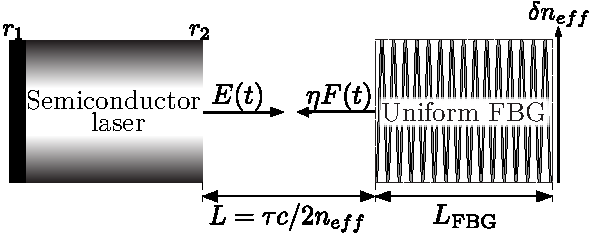
\includegraphics[width=\linewidth]{Images/FBG_setup_dneff_only_1col.pdf}
    \caption{Sketch of an optical fiber with an FBG written along its length.}
    \label{fig:FBG_setup}
\end{figure}
%
\par
%
An FBG is defined as a periodic modulation $\delta n_{eff}(z)$ of the refractive index with period $\Lambda$ along a fibre of length $L_\text{FBG}$.
The number of gratings in an FBG is therefore $N = L_\text{FBG}/\Lambda$. The most general form of this periodic modulation is
%
\begin{equation}
\label{eq:dneff}
    \delta n_{eff}(z) = \dnbar(z) \left[ 1 + v \cos{\left( \frac{2 \pi}{\Lambda} z + \phi(z) \right)} \right].
\end{equation}
%
Here, $\dnbar(z)$ describes the envelope of the periodic modulation along $L_\text{FBG}$; for example, $\dnbar(z) \sim e^{-z^2}$ yields a Gaussian refractive index profile. 
This flexibility allows tailoring of the spectral response through modulation depth and phase, directly influencing the accessible ECM structure.
In addition to the envelope, $v$ denotes the fringe visibility of the index modulation, and $\phi(z)$ allows variation of the grating period along the fibre, enabling different frequencies to be reflected at different positions.
%
\par
%
Light propagating in the fibre and interacting with the FBG undergoes diffraction when its wavelength is close to the design wavelength, $\lambda_D = 2 n_{\text{eff}} \Lambda$.
It is typically assumed that the light undergoes only first-order diffraction, which dominates in FBGs, so that a single propagating mode is considered; higher-order diffraction is negligible under standard design conditions.
In this case, using coupled-mode theory and the synchronous approximation, one can derive coupled first-order differential equations describing the interaction between the forward- and backward-propagating waves, $A(z)$ and $B(z)$, respectively.
For further details, see \cite{erdogan1997fiber} and references therein.
%
\begin{equation}
\label{eq:wave_eqs}
    \begin{aligned}
        \frac{dR}{dz} &= i \hat{\sigma} R(z) + i \k S(z), \\
        -\frac{dS}{dz} &= i \hat{\sigma} S(z) + i \k R(z),
    \end{aligned}
\end{equation}
%
with $R(z) = A(z) \exp{ \left( -i \left( \phi/2 -\delta z \right) \right) }, \; S(z) = B(z) \exp{ \left( -i \left( \phi/2 + \delta z \right) \right) }$.
The parameters $\delta$, the wavevector mismatch, $\kappa$, the alternating-current (AC) coupling coefficient, and $\hat{\sigma}$, the direct-current (DC) self-coupling coefficient, are given by
%
\begin{align}
    \label{eq:delta}
    \delta &= 2 \pi \neff \left( \frac{1}{\lambda} - \frac{1}{\lambda_D} \right) \\
    \label{eq:kappa}
    \k &= \frac{\pi}{\lambda} v \dnbar(z)\\
    \label{eq:sigma}
    \hat{\sigma} &= \frac{2\k}{v} + \delta -\frac{1}{2}\frac{d\phi}{dz}
\end{align}
%
Since $\k$ and $\hat{\sigma}$ generally depend on $z$, \eqref{eq:wave_eqs} cannot in general be solved analytically, but they can be readily solved numerically once $\Lambda$, $n_{\text{eff}}$, $\dnbar(z)$, $\phi(z)$, and $L_\text{FBG}$ are specified.
%
\par
%
At this point, all the necessary ingredients are in place to calculate the key characteristic of an FBG—its reflectivity spectrum $\rho(\w)$.
Physically, the primary interest lies in the reflection spectrum of light reflected at the front FBG interface, assuming no reflection from the back interface.
Therefore, \eqref{eq:wave_eqs} is typically solved by setting $z = 0$ at the midpoint of the FBG, imposing boundary conditions $R(-L_\text{FBG}/2) = 1$ and $S(L_\text{FBG}/2) = 0$, and integrating backwards from $L_\text{FBG}/2$ to $-L_\text{FBG}/2$. The amplitude reflection coefficient is then given by
%
\begin{equation}
\label{eq:rho}
    \rho = \frac{S(-L_\text{FBG}/2)}{R(-L_\text{FBG}/2)}
\end{equation}
%
which defines the reflectivity spectrum $\rho(\omega)$.
Although \eqref{eq:wave_eqs} must generally be solved numerically and closed-form expressions for $\rho(\omega)$ are rarely available, certain standard grating designs such as uniform or raised-cosine-apodised gratings admit analytic solutions and provide valuable insight into the typical properties of FBG reflection spectra.
Among the different grating profiles, the simplest and most widely studied is the uniform grating.
%
%
\subsubsection*{Uniform FBG reflection spectra $\rho_\text{Bragg}(\w)$}
\label{subsubsec:FBG_feedback}
%
The uniform FBG serves as the canonical case for analysis, characterised by constant period and constant modulation depth.
It admits analytic solutions that not only reveal the fundamental characteristics of FBG reflection spectra but also serve as a reference for more complex grating designs.
In this case, the grating chirp satisfies $\sfrac{d\phi}{dz} = 0$ and the apodisation is constant, $\dnbar = \text{const.}$, so that the grating index variation given by \eqref{eq:dneff} reduces to a sine wave, as shown in Figure~\ref{fig:FBG_setup}.
Therefore, $\k$ and $\hat{\sigma}$ are constant in $z$, which allows the reflectivity spectrum $\rho(\omega)$ to be obtained analytically by solving \eqref{eq:wave_eqs} and then evaluating \eqref{eq:rho}.
%
\begin{equation}
\label{eq:uniform_rho}
    \rho = \frac{-\k \sinh\left( L_\text{FBG}\right)}{\hat{\sigma} \sinh\left(\gamma L_\text{FBG}\right) + i\gamma \cosh\left(\gamma L_\text{FBG}\right)}
\end{equation}
%
where $\gamma = \sqrt{\k^2 - \hat{\sigma}^2}$. Several key features of the reflection spectrum $\rho(\omega)$ are most clearly visualised by plotting it as a function of normalised frequency while varying $\kappa L_\text{FBG}$ for a fixed $N$ \cite{erdogan1997fiber}.
%
\begin{equation*}
    \frac{\omega}{\omega_\text{max}} = 1 + \frac{\hat{\sigma} L_\text{FBG}  }{\pi N}
\end{equation*}
%
Figure~\ref{fig:uniform_spectra_varykL} shows representative amplitude reflectivity and phase spectra for uniform gratings, plotted against angular frequency. 
The gratings are centred at the common laser wavelength of 1550 nm, with $\kappa L_\text{FBG} \in {0.5, 2, 5}$ and a fixed $N = 5000$, chosen to illustrate weak, moderate, and strong coupling regimes.
Increasing $N$ (and thus $L_\text{FBG}$) results in a narrower reflection bandwidth, whereas decreasing $N$ (and thus $L_\text{FBG}$) produces a broader one, provided that $\kappa L_\text{FBG}$ remains constant.
The reflection spectrum consists of a main lobe and a series of side lobes, separated by reflection zeros that are symmetrically spaced in wavelength on either side of the main lobe.
For gratings with low $\kappa L_\text{FBG}$, such as 0.5, the main lobe has a bandwidth, defined as the interval between its reflection zeros, that is twice the width of the side lobes \cite{erdogan1997fiber}.
Evidently, increasing $\kappa L_\text{FBG}$ increases the grating's maximum reflectivity and also broadens the main-lobe bandwidth while narrowing that of the side lobes.
Additionally, the time delay is approximately constant for low reflectivities but becomes increasingly distorted as $\kappa L_\text{FBG}$ increases.
%
\begin{figure}[!t]
    \includegraphics[width=\linewidth]{Images/Uniform_varying_kL_Rtau.pdf}
    \caption{Examples of magnitude and phase of uniform FBG reflection spectra with varying dimensionless grating strength $\k L_\text{FBG} \in [0.5, 2, 5]$ and constant number of grating periods $N=5000$.}
    \label{fig:uniform_spectra_varykL}
\end{figure}
%
\par
%
Since $\kappa$ and $\hat{\sigma}$ depend only on $\lambda$ and the prescribed grating parameters, the reflected amplitude $|\rho|$ and phase $\arg(\rho)$ can be directly plotted against frequency by substituting \eqref{eq:kappa} and \eqref{eq:sigma} into \eqref{eq:uniform_rho}.
Figure~\ref{fig:uniform_spectra_varying_L_dneff} shows examples of reflection spectra of uniform FBGs plotted against frequency, with the design frequency given by
%
\begin{equation}
    \w_D = \frac{\pi c}{\Lambda n_{eff}^2}
\end{equation}
%
highlighted to demonstrate the intrinsic frequency shift in the spectrum. The reflection spectrum of a uniform grating has a maximum reflectivity
%
\begin{equation}
\label{eq:rmax}
    R \equiv |\rho_\text{max}| = \tanh{(\k L_\text{FBG})}
\end{equation}
%
centred at the Bragg frequency $\omega_\text{max}$,
%
\begin{equation}
\label{eq:wBragg}
    \w_\max = \frac{\w_D}{\left( 1 + \frac{\dnbar }{\neff}\right)}
\end{equation}
%
corresponding to the peak reflectivity.
We note that $R$ is more commonly used to denote reflected power rather than reflected amplitude; however, the present notation is adopted for clarity in later sections.
The phase at $\omega_\text{max}$ is $\sfrac{\pi}{2}$ for all uniform gratings, while the reflection zeros are symmetric about $\omega_\text{max}$. 
The first zeros on either side of the main lobe occur at $\omega_\text{max} \pm \omega_z$, where
%
\begin{equation}
\label{eq:wz}
    \wz = \w_\max \sqrt{\left( \frac{\dnbar}{2 \neff} \right)^2 + \frac{1}{N^2} }
\end{equation}
%
and the phase of the reflection spectrum shifts by $2\pi$ between these zeros.
Outside the main lobe, the reflectivity peaks of the side lobes decay exponentially, with a $\pi$ phase change across each lobe.
%
\begin{figure}[!t]
    \includegraphics[width=\linewidth]{Images/Uniform_varying_L_dneff.pdf}
    \caption{Examples of the magnitude and group delay of uniform FBG reflection spectra, illustrating the effect of varying $\dnbar$ and $L_\text{FBG}$. 
    The nominal case (black curves) corresponds to $\dnbar = 5\e{-5}\neff$ and $L_\text{FBG} = 2.64,\text{mm}$; in (a) the grating length is doubled to $L_\text{FBG} = 5.28,\text{mm}$, and in (b) the index change is doubled to $\dnbar = 1\e{-4}\neff$.}
    \label{fig:uniform_varying_L_dneff}
\end{figure}
%
\par
%
Figure~\ref{fig:uniform_varying_L_dneff}(a) shows that doubling $L_\text{FBG}$ increases $R$ because more grating periods contribute to reflection, reducing transmission. 
At the same time, the bandwidth of each lobe is halved, while the offset from the design frequency remains unchanged. 
In contrast, doubling $\dnbar$, as shown in (b), again increases $R$, but now the offset from the design frequency increases while the bandwidth remains unchanged. 
Since these two parameters govern the three key spectral features—offset, maximum reflectivity, and bandwidth—one cannot vary a single feature independently. 
Instead, compensation requires adjusting the grating period $\Lambda$, which shifts $\w_\max$ while leaving $\wz$ and $R$ essentially unchanged. 
This holds because laser centre frequencies are in the THz range, whereas the frequency offset is at most in GHz, so $\w_\max}/\w_D = \Lambda_D/\Lambda_{\max} \approx 1$.
Using this approximation, together with \eqref{eq:wBragg} and \eqref{eq:wz}, $\dnbar$, $L_\text{FBG}$, and $\Lambda$ can be calculated sequentially.
%
\begin{align}
\label{eq:spec2phys}
    \dnbar &\approx \frac{2\wz}{\w_c} \frac{\neff}{\sqrt{1 + \left(\frac{\pi}{\arctanh{(R)}} \right)^2}}
    \\
    \Lambda &= \frac{\pi c}{\w_c \neff (\neff +\dnbar)}
    \\
    L &= \frac{\Lambda}{\sqrt{\left( \frac{\wz}{\w_c} \right)^2 - \left( \frac{\dnbar}{2\neff} \right)^2}}
\end{align}
%
For example, if a uniform grating with a spectral response corresponding to $\w_c = 1.216\e{15}\; \text{rad s}^{-1}$, $\wz = 1\e{10}\; \text{rad s}^{-1}$, and $R = 0.5$ is desired, 
\eqref{eq:spec2phys} provides grating parameters $\dnbar= 4.2111838\e{-6}$, $\Lambda = 3.6494583\e{-7}\,\text{m}$, $L = 0.0444578955\,\text{m}$, 
which gives excellent agreement to the desired spectral response as shown in Figure~\ref{fig:spec2phys}.
%
%
\section*{FBG distributed feedback}
\label{sec:FBG_feedback}
%
Given the significant spectral advantages of FBGs for FOF and the straight-forward integration of FBGs into fiber optic semiconductor laser systems, 
investigations into their influence on the dynamics of external feedback semiconductor laser systems is of great interest. 
A sketch of the laser system under external feedback from an FBG is shown in Figure~\ref{fig:FBGF}. 
As demonstrated in the previous section, the reflectivity spectrum of FBGs can be rather complex. 
As an FBG in essence acts as a filter, the term $F(t)$ will be given by \eqref{eq:FOF} with $\rho(\w) = \rho_\text{Bragg}(\w)$. 
This term can alternatively be written as a convolution in the time domain,
%
\begin{equation}
    \label{eq:convolution}
     F(t) = e^{-i C_p} \tilde{\rho}_\text{Bragg}(t) \otimes E(t-\tau)
\end{equation}
%
where $\tilde{\rho}_\text{Bragg}(t)$ is the impulse response of the FBG with respect to the Bragg resonance frequency. 
Analytic expressions do not exist for the impulse response, even for simple gratings, and must therefore be calculated numerically through fast Fourier transforms (FFTs), for example. 
The requirement of numerically calculating $F(t)$ limits the analysis to numerical integration of solutions for $(E(t),N(t))$, and calculating properties of resulting time series, 
such as maximal Lyapunov exponents (MLEs) or spectral characteristics such as signal dispersion. 
Despite the obvious computational and analytical difficulties associated with this feedback term, 
research has been conducted into uniform FBG feedback using the convolution representation for $F(t)$ \cite{li2012distributed, li2015chaotic, li2020stable, jiang2021characterizing, skenderas2021feedback, skenderas2024impact}. 
In several studies, an expression for $\rho(\w)$ separates the reflection spectrum and detuning, allowing the detuning to be varied continuously while keeping the reflectivity spectrum shape constant. 
In this case, the reflected signal has the form,
%
\begin{equation*}
    F(t) = \eta e^{-i C_p} [\tilde{\rho}_0(t) e^{i \wB t}] \otimes E(t-\tau)
\end{equation*}
%
where $\tilde{\rho}_0$ is centred at the laser free-running frequency, while the detuning $\wB$ is an independent parameter. 
Although this form for the reflectivity distribution allows one to vary a single feature of the reflectivity distribution, as discussed in \ref{subsec:FBG_feedback}, the detuning and distribution shape intrinsically depend on each other, 
meaning that all grating parameters $\dnbar, \Lambda, L$ must be simultaneously adjusted in order to continuously detune over a constant distribution shape \cite{skenderas2024impact}. 
These parameters can be calculated for example through \eqref{eq:spec2phys}. 
Similarly, the distribution width and maximum reflectivity (occurring at $\w_c$) can only be independently varied through simultaneously varying all grating parameters.
%
\par
%
As numerical investigations only allow limited insights into the underlying dynamics of FBG feedback, initial numerical investigations focused on the potential of FBG feedback to produce high-quality chaotic signals. 
This is of research interest as chaotic signals produced by lasers subject to external feedback are used in a number of applications such as high-speed optical random bit generation \cite{uchida2008fast} and chaos-based secure communication \cite{annovazzi2008secure}. 
It was demonstrated that FBG feedback is more effective than conventional mirror feedback in suppressing the time-delay signature (TDS) associated with chaos generation in semiconductor lasers. 
TDS can limit the encryption capabilities of chaotic signals generated lasers subject to external feedback, as powerful autocorrelation algorithms can use a signal's TDS to partially or fully decrypt the signal \cite{rontani2007loss}. 
The improvement in TDS suppression was generally attributed to the time-distributed reflections provided by the FBG, `spreading out' the effective time delay of the chaotic signal \cite{li2012distributed}. 
Further, it was observed that TDS suppression improves as the bandwidth of the FBG decreases. This is linked to the increase in dispersion of the reflection group delay, which plays a crucial role in the dynamics of the laser. 
Notably, the length of the FBG does not significantly affect this suppression. 
Although narrower FBG bandwidth enhances chaotic signal TDS suppression, the size of parameter regions that exhibit chaos decrease, being replaced by regions of stable period-1 periodic orbits, 
in agreement with analyses of FOF \cite{li2020stable}, although it was demonstrated that in some cases, 
chaos can be induced by FBG feedback for lower time delays than what is possible using COF. 
Further investigations showed that optimal TDS suppression is achieved when the FBG is positively detuned from the laser frequency. 
The preference for positive detuning is attributed to the red-shifting of the laser cavity due to the anti-guidance effect \cite{li2015chaotic}. 
%
%From a dynamical systems perspective, these initial numerical investigations raised interesting questions on why there is an intrinsic asymmetry about the FBG spectrum in laser stability for positive or negative detuning and whether the laser frequency 
%
\par
%
The convolution representation for $F(t)$ under FBG feedback can alternatively be written as a distributed delay term. Using the definition of the convolution,
%
\begin{align*}
    \tilde{\rho}(t) \otimes E(t-\tau)
    &= \int_{-\infty}^{\infty} \tilde{\rho}(t-s) E(s-\tau) ds \\
    &= \int_{-\infty}^{t+\tau} \tilde{\rho}(t-s) E(s-\tau) ds
\end{align*}
%
as $E(s-\tau)=0$ for $s>t+\tau$. Now, choosing the lower bound $t-T$ so that $\tilde{\rho}(s) \approx 0 \; \forall \; s>T$.
%
\begin{equation*}
    \tilde{\rho}(t) \otimes E(t-\tau) \approx \int_{t-T}^{t+\tau} \tilde{\rho}(t-s) E(s - \tau) ds
\end{equation*}
%
This equivalent expression for $F(t)$ has been used in further numerical studies on the use of chirped FBGs (CFBGs), 
which are of interest in TDS suppression due to their enhanced dispersion characteristics compared to the previously explored uniform FBGs \cite{wang2017time, wang2019key, wang2023critical, chao2020permutation}. 
An illustration of the index profile of CFBGs is given in Figure~\ref{fig:dneff}(d). 
As there are no analytic expressions for a chirped reflectivity spectrum compared to a uniform one, \eqref{eq:wave_eqs} must be solved numerically, further increasing computational complexity. 
The impulse response $\tilde{\rho}(t)$ involved in the distributed feedback is calculated through FFTs as done in previous investigations. 
Investigations into CFBG feedback demonstrated enhanced TDS compared to uniform FBG feedback, eliminating TDS without requiring amplification, simplifying system configuration.
%
\par
%
More recently, investigations have gone beyond studying chaotic signal generation but similar to the previous analyses, the convolution representation for $F(t)$, restricted computations to basic time series generation. 
\Skenderas \textit{et al.} observed that the location of the zeros of the reflectivity spectrum, can strongly influence laser stability. 
They demonstrated that these stability fluctuations are likely due the damping of relaxation oscillations (ROs) when the zeros of the FBG reflectivity spectrum is aligned with the laser's RO frequency ($\w_{RO}$) side lobes. 
These stability fluctuations were found by tracking the required feedback rate to produce a Hopf bifurcation, that is, where constant intensity emission begins to periodically fluctuate, for increasing the FBG length which in turn decreases FBG bandwidth. 
As changing FBG length changes its reflectivity, the other FBG parameters are required to be adjusted to ensure a constant reflectivity. 
Asymmetry in stability fluctuations were observed for frequency detuning relative to the Bragg wavelength, as was the case in previous studies \cite{li2012distributed}, but alternatively attributed to the frequency-dependent phase shift induced by the FBG \cite{skenderas2024impact, skenderas2021feedback}. 
This gives further indication that the observed asymmetrical behaviour with respect to detuning emerges as an intrinsic characteristic of FBG feedback. Overall, the numerical simulations reveal that FBG feedback shares many features with FOF. 
However, the precise shape, location of reflection zeros, and, most notably, the phase of the FBG introduce additional complexity. 
%
\par
%
While the representation of $F(t)$ as a convolution has been shown to provide some limited insights into FBG feedback, an alternative form for $F(t)$ has been shown to allow deeper analyses into its associated dynamics. 
The case of FBG feedback subject to strong feedback was considered in a series of papers by Naumenko \textit{et al.} \cite{naumenko2003characteristics, naumenko2004slow, besnard2002intensity}. 
The modified rate equations used in the analysis are based on a model first proposed in 1989 \cite{rong1989improved} describing strong feedback due to a plain mirror. 
They replace the feedback term $\eta e^{-i C_p} E(t-\tau)$ in the LK rate equations with the term $E(t) \ln{\left[ E_r(t) / E(t) \right]}$ where $E_r(t)$ accounts for the multiple EC reflections caused by the strong COF, 
similar to \eqref{eq:multiple_EC} by defining
%
\begin{equation*}
    E_r(t) = E(t) + \frac{R_2^2 - 1}{R_2^2} \sum_{n=1}^\infty (-R_2 R)^n e^{-i n C_p} E(t-n \tau)
\end{equation*}
%
Indeed, truncating this expression for $F(t)$ to first order reduces to single reflection feedback. Taking the Taylor expansion of the logarithm,
%
\begin{equation*}
    \begin{aligned}
        &E(t) \ln{\left[ \frac{E_r(t)}{E(t)} \right]} = \sum_{n=1}^\infty \frac{(-1)^{n-1}}{n}\left( \frac{E_r(t)}{E(t)} - 1\right)^n \\
        &\,\overset{n=1}{\approx} E(t)\left( \frac{E(t) + \frac{R_2^2 - 1}{R_2^2}(-R_2 R)e^{-i C_p} E(t - \tau) - E(t)}{E(t)} \right)\\
        &\;\;= \eta e^{-i C_p} E(t - \tau)
    \end{aligned}   
\end{equation*}
%
as desired.
Reflection due to an FBG can be modelled by modifying this expression to account for the spectral filtering $\rho_{\text{Bragg}}(\w)$ of the grating. 
Multiple reflections given by the terms $(R_2 R)^n e^{-i n C_p} E(t-n \tau)$ are now replaced by terms given by \eqref{eq:FOF}, see Appendix~\ref{sec:multiple_EC_nondim} for details. 
Through the use of Green's functions, an expression for the ECMs of the system can be derived, allowing for significantly deeper insights into the dynamics compared to the convolution method discussed previously. 
It was shown that under weak feedback, the stationary ECM states are mostly confined to the main lobe of the gratings reflectivity spectrum, while the MGM is shifted close to $\wB=0$, 
identical to the results presented by Yousefi and Lenstra in the case of FOF. 
They additionally identified `satellite' ECMs, for narrow bandwidth FBGs, separated from the central ECM ellipse by the zeros of the main lobe. 
It is shown that under strong feedback conditions that narrow filters lead to the excitation of additional solutions confined to the side lobes of the FBG frequency response. 
Although numerical integration of the presented system can be performed, and stationary states calculated, 
the complexity of $F(t)$ prevents the use of advanced bifurcation tools such as numerical continuation and stability analysis of the stationary solutions, clouding the underlying dynamics induced by the frequency-dependent FBG reflection. 
%
\par
%
The similarities in the results of Naumenko \textit{et al.} to work on FOF is fairly evident when one considers a single reflection. 
Carrying out the same first-order approximation on this feedback term yields an equivalent feedback term as used in the original FOF definition considered by Yousefi and Lenstra with $\rho(\w) = \rho_\text{Bragg}(\w)$. 
See Appendix~\ref{sec:multiple_EC_nondim} for further details. 
Therefore, it is natural to ask if there is a an approximation to $\rho_\text{Bragg}(w)$ which captures its key frequency-dependent reflection effects while enabling the feedback term $\eta F(t)$ to be reduced to DDEs which amenable to advanced bifurcation analysis.
% !TeX root = ../main.tex
\section{Uniform FBG modelling through discretised reflections}
\label{sec:FBG_discretised}
%
To overcome the limitations of convolution-based models and the absence of analytical ECM analyses, we seek a representation of FBG feedback that links directly to physical parameters while preserving the mathematically tractable delay–differential structure of the LK equations.
One promising route is to approximate the distributed reflection process directly in the time domain through discretised reflections.
Although most approaches in the literature begin with the spectral response of the grating, the reflection spectrum can also be modelled by approximating the grating as a sequence of discrete layers, each contributing a reflection and transmission event \cite{poladian2000simple, ghiringhelli2002time, feced2002efficient, skaar2001synthesis}. 
This construction amounts to a discretised version of the impulse response $\tilde{\rho}(t)$ that would otherwise be obtained from $\rho(\omega)$ by an inverse Fourier transform. 
By considering all optical paths that re-emerge from the FBG after a delay of $\tau_k$, the impulse response can be written as a weighted sum of delta functions,
%
\begin{equation}
    \label{eq:dicretised_impulse}
    \tilde{\rho}(t) = \sum_{k=0}^N h_r(k)\, \text{Dirac}(t-\tau-\tau_k)
\end{equation}
%
which we refer to as the discretised impulse response.
Physically, $h_r(k)$ encodes the effective amplitude of all paths contributing to the delayed signal emerging after a time delay $\tau_k$ as illustrated in Figure~\ref{fig:discretised_FBG}(a).
For non-uniform gratings, the average refractive index varies along the structure, requiring distinct refractive indices $n_i$ and corresponding transmission and reflection coefficients $t_{i,i+1}$ and $r_{i,i+1}$ to be computed for each layer.
This approach has been shown to recover the spectral response $\rho(\omega)$ with high accuracy \cite{ghiringhelli2002time}.
Here, however, we focus on the simpler case of uniform FBGs, where the average index is constant along the grating, so that all layers are identical.
This simplification yields a particularly transparent formulation of the feedback term $F(t)$ in terms of the coefficients $h_r(k)$, without requiring explicit reference to the full spectral response.
%
\par
%
We will show in the following that an approximate model for this discretised-reflection framework retains the analytic tractability of the Lorentzian FOF model discussed in section~\ref{subsec:FOF}, while also faithfully reproducing the reflection spectrum of uniform FBGs across a broad frequency range. 
This combination of accuracy and simplicity opens the way to both closed-form equations for cavity modes, efficient numerical integration, and advanced numerical methods such as continuation.
%
%
\subsection{Uniform FBG discretised reflection model derivation}
\label{subsec:FBG_discretised_derivation}
%
\begin{figure}[!t]
    \centering
    
    \begin{overpic}[width=0.95\linewidth]{Images/discretised_reflections.pdf}
        \put(-1,60){(a)}
    \end{overpic}\\[0.5em]
    \begin{overpic}[width=0.95\linewidth]{Images/single_reflection_tk.pdf}
        \put(-1,60){(b)}
    \end{overpic}
    
    \caption{(a) Illustration of the first six layers in the slab decomposition of a uniform FBG, showing transmission and reflection coefficients between adjacent layers ($j=i+1$). 
    (b) Illustration of the contribution to the reflected field arising solely from reflection at the $k^{\text{th}}$ layer, corresponding to the $k^{\text{th}}$ delayed signal.}
    
    \label{fig:discretised_FBG}
\end{figure}
%
\begin{figure}[!t]
    \centering
    
    \hspace{0.04cm}
    \begin{overpic}[width=\linewidth]{Images/R_tau_discretised_accuracy.pdf}
        \put(-4,93){(a)}
        \put(-4,48){(b)}
    \end{overpic}

    \caption{A comparison between the exact (solid lines) total reflection \eqref{eq:R_exact} and discretised (dashed lines) total reflection \eqref{eq:R_approx} is shown in (a), and the exact effective delay \eqref{eq:tau_exact} and discretised delay expectation \eqref{eq:tau_approx} is shown in (b) as functions of the normalised refractive index variation $\dn$ for varying $N \in [10,100,1000,10000]$.}

    \label{fig:R_approximations}
\end{figure}
%
We model the reflection response of a uniform FBG as arising from partial reflections at evenly spaced boundaries across $N$ layers of the grating. 
The grating has a uniform average refractive index $\neff$, while each boundary introduces the same transmission coefficient $t$ and reflection coefficient $r$, determined by the normalised refractive index variation $\dn \equiv \dnbar/\neff$. 
Further, the constant $\neff$ ensures that the round-trip time $\dt$ is constant across all layers so that $\tau_k = k \, \dt$. 
For tractability, we consider only the dominant propagation paths that undergo a single reflection at the $(k-1)^\text{th}$ layer. 
A contribution from such a path re-emerges from the grating after a time delay of $k\,\dt$, as sketched in Figure~\ref{fig:discretised_FBG}(b). 
In this way, the discretised model mirrors the idea of an impulse response composed of delayed replicas of the input field, but expressed in terms of individual layer reflections.
%
\par
%
For the discretised formulation to be meaningful, it must reproduce the essential characteristics of a uniform FBG, most importantly the total reflectivity $R$, while linking the effective coefficients $r$ and $t$ to the physical parameters of the grating.
The exact reflectivity of a uniform FBG at its Bragg frequency, given by \eqref{eq:rmax}, can be written as
%
\begin{equation}
\label{eq:R_exact}
R_\text{exact} = \tanh{\left(\frac{\pi}{2}\frac{N \, \dn}{1+\dn} \right)}.
\end{equation}
%
A key observation is that this expression is very well approximated by the simpler form
%
\begin{equation}
\label{eq:R_approx}
R_\text{approx} = 1 - \left(1 - \dn \right)^{2N},
\end{equation}
%
as shown in Figure~\ref{fig:R_approximations}(a), where both forms are plotted as a function of $\dn$ for different $N$.
The close agreement confirms that the discretised model reproduces the correct scaling of reflectivity with both modulation depth and grating length.
To connect this approximation to a reflection model, we represent the signal emerging from the front facet after a time delay $k \, \dt$ as having passed through $k-1$ transmissive layers before being reflected at the $k^\text{th}$ layer, with no further attenuation thereafter.
The corresponding contribution is
%
\begin{equation}
\label{eq:hr1}
h_r(k) = t^{k-1} r,
\end{equation}
%
where $t$ and $r$ denote the effective transmission and reflection coefficients.
To ensure consistency with \eqref{eq:R_approx}, these coefficients must reproduce the total reflectivity when all delayed reflections are summed.
Rewriting \eqref{eq:R_approx} as a geometric series,
%
\begin{align*}
R_\text{approx} &= 1 - (1-\dn)^2 + (1-\dn)^2 - \dots \\
&\hspace{1em} - (1-\dn)^{2N-2} + (1-\dn)^{2N-2} - (1-\dn)^{2N} \\
&= \left( 1-(1-\dn)^2 \right)\left( 1 + (1-\dn)^2 + \dots + (1-\dn)^{2N-2} \right) \\
&= (1-(1-\dn)^2)\sum_{k=1}^{N} \left((1-\dn)^2\right)^{k-1},
\end{align*}
%
we arrive at an expression that is exactly reproduced by \eqref{eq:hr1} if we define
%
\begin{align}
\label{eq:tr}
t &\equiv (1-\dn)^2, \\
r &\equiv 1-(1-\dn)^2.
\end{align}
%
\par
%
Because FBGs act as distributed reflectors, it is not sufficient for the discretised model to match only the total reflectivity; it should also capture the effective delay of the structure, which represents how the reflected energy is distributed in time across multiple paths.
This can be tested by comparing the average delay predicted by the discrete reflections, $E[\tau_\text{FBG}]$, with the effective delay $\tau_{eff}$ derived directly from the exact reflection spectrum \cite{barmenkov2006effective}.
The effective time delay can be written in terms of the layer round-trip time $\dt = 2 \Lambda \neff/c$ as
%
\begin{equation}
    \label{eq:tau_exact}
    \tau_{eff} = \frac{R_\text{exact} \dt}{\pi \, \dn}.
\end{equation}
%
The expected delay of the discretised reflections $E[\tau_\text{FBG}]$ is calculated as the weighted average of the delays of all the reflected signals, where the weights are the amplitudes of the reflected signals. 
Mathematically,
%
\begin{equation*}
    E[\tau_\text{FBG}] = \frac{r \sum_{k=1}^{N} t^{k-1} (k-1)\dt}{r \sum_{k=1}^{N} t^{k-1}}.
\end{equation*}
%
The sum in the denominator is simply the sum of a geometric sequence, having a closed form
%
\begin{equation*}
    \sum_{k=1}^{N} t^{k-1} = \frac{1-t^N}{1-t}.
\end{equation*}
%
The sum in the numerator can be evaluated efficiently by noting that it can be written in terms of a derivative w.r.t. $t$ of the numerator. That is,
%
\begin{equation*}
    \sum_{k=1}^{N} t^{k-1} (k-1) = t \, \frac{\partial}{\partial t} \sum_{k=1}^{N} t^{k-1} = \frac{t(1-t^N)}{(1-t)^2} - \frac{N t^N}{1-t}.
\end{equation*}
%
The effective delay then simplifies to
%
\begin{equation}
    \label{eq:tau_approx}
    E[\tau_\text{FBG}] = \dt\left[ \frac{t}{1-t} - \frac{N t^N}{1-t^N} \right].
\end{equation}
%
\par
%
Figure~\ref{fig:R_approximations}(b) compares the effective delay $\tau_{eff}$ with the expected delay $E[\tau_\text{FBG}]$ of the discretised model, plotted as a function of $\dn$ for different $N$.
The comparison shows that the discretised model reproduces the effective delay with high accuracy, matching closely at small $\dn$ and diverging only gradually at larger values.
Although the accuracy of delay and reflectivity vary differently with $\dn$, the model reproduces both with sufficient consistency to remain reliable across the full parameter range.
%
\par
%
A key property of the coefficients in \eqref{eq:tr} is that they satisfy $r+t=1$, resembling the familiar balance between reflection and transmission. 
Unlike true Fresnel coefficients, however, these are effective coefficients: they subsume the cumulative effect of multiple internal transmissions and reflections into a single pair of parameters. 
In doing so, they preserve the correct scaling of reflectivity with $\dn$ and $N$ while providing a compact, physically transparent description that is straightforward to use in dynamical models such as the LK equations. 
%
\begin{equation}
    \label{eq:discretised_impulse_full}
    \tilde{\rho}(t) = (1-t)\sum_{k=0}^{N-1} t^k \, \delta(t-\tau-k\dt)\, e^{-i k \wB \dt},
\end{equation}
%
where each term corresponds to a contribution that has traversed $k$ transmissive layers, been reflected once, and accumulated an additional phase $e^{-i k \wB \dt}$ from propagation through the grating. 
Since the LK equations are defined relative to the free-running laser frequency (so that $\wZ=0$), the parameter $\wB$ naturally enters as the detuning of the grating's Bragg frequency. 
This highlights that the FBG acts as a weighted superposition of delayed, phase-shifted replicas of the input field. 
We remark that if backward transmission were explicitly included, alternative but mathematically consistent definitions of $r$ and $t$ could be derived, though the present choice yields cleaner expressions for the analysis that follows.
%
\par
%
With this foundation, the feedback term $F(t)$ follows directly as the convolution of the field with \eqref{eq:discretised_impulse_full}, consistent with earlier convolution-based formulations \cite{skenderas2024impact,skenderas2021feedback,li2012distributed,li2015chaotic,li2020stable}:
%
\begin{align*}
F(t) &= e^{-i C_p} E(t) \otimes \tilde{\rho}(t) \\
&\approx r e^{-i C_p} \sum_{k=0}^{N-1} t^k E(t) \otimes \delta(t-\tau-k\,\dt) e^{-i k \wB \dt} \\
F(t) &\approx (1-t) e^{-i C_p} \sum_{k=0}^{N-1} t^k E(t-\tau-k\,\dt) e^{-i k \wB \dt}.
\end{align*}
%
\par
%
Taken together, these results establish the discretised-reflection formulation as a reliable and practical approximation to FBG feedback. 
Crucially, it preserves the analytic tractability of the LK system while embedding essential features of grating physics, thereby enabling both efficient time-domain simulations and deeper analytical exploration of cavity modes. 
The central parameter $t$, which enters the LK equations, is determined directly from the target reflectivity via \eqref{eq:R_approx}:
%
\begin{equation}
\label{eq:discretised_t}
t = \big(1-R\big)^{1/N},
\end{equation}
%
providing a transparent connection between physical grating design and the discrete-feedback model. 
This link ensures that the formulation is not only computationally convenient but also grounded in experimentally tunable parameters, making it a robust foundation for the analyses that follow.
%
\par
%
With both reflectivity and effective delay validated, the discretised model can now be embedded directly into the LK equations, which take the form
%
\begin{equation}
\label{eq:LK_discretised}
    \begin{aligned}
        \frac{d E}{d t} = (1 &+i \a) N(t) E(t) + \\
                        &\quad \eta (1-t) e^{-i C_p} \sum_{k=0}^{N-1} t^k E(t-\tau-k\, \dt) e^{-i k \wB \dt} \\
        T \frac{d N}{d t} &= P-N(t)-(1+2 N(t))|E(t)|^2.
    \end{aligned}
\end{equation}
%
Unlike convolution-based models, this formulation reduces the feedback to a finite sum of discrete delays, preserving the DDE structure for ECM analysis and continuation, while also providing a platform to explore the spectral properties of the system through its mode structure.
%
%
\subsection{EGM modes of the discretised reflection model}
\label{subsec:EGM_discretised}
%
A natural first step in assessing any feedback model is the calculation of its cavity modes, since these steady-state solutions provide the `backbone' of the system and reveal how the feedback reshapes the laser’s mode structure.
In the COF and FOF cases, mode calculations (ECMs and EFMs, respectively) have been central to validating both the physical realism and the analytical tractability of the models.
For the discretised FBG reflection model, the corresponding external grating modes (EGMs) serve the same purpose: they provide a direct spectral interpretation of the formulation, constitute the first point of comparison with the known reflection properties of uniform FBGs, and act as benchmarks for demonstrating that the model captures not only physical but also spectral characteristics of FBG feedback.
Beyond this role in validation, EGMs also structure much of the system’s dynamics and stability \cite{rottschafer2007ecm}, and once stable solutions are identified they can be systematically continued in parameters using specialised DDE continuation software such as \texttt{DDE-BifTool}.
%
\par
%
The EGMs take the form $(E(t), N(t)) = (E_s e^{i\w_s t}, N_s)$ with $E_s, \w_s, N_s \in \mathbb{R}$, corresponding to a laser field oscillating at a shifted frequency $\w_s$ with constant amplitude $E_s$ and inversion $N_s$.
Physically, $\w_s$ represents the detuning of the locked field from the solitary laser frequency $\w_0$.
Substituting this ansatz into \eqref{eq:LK_discretised} yields an implicit equation for the allowed EGM frequencies.
To this end, we first separate the resulting complex equation into its real and imaginary parts by expanding the exponentials, giving
%
\begin{align*}
    i \w_s = (1+i \a) N_s &+ \eta (1-t) \big(\cos{(\phi_\text{E})} -i\sin{(\phi_\text{E})}  \big) \times \\ 
                        &\left( \sum_{k=0}^{N-1} t^k \cos{(k\phi_\text{F})} - i \sum_{k=0}^{N-1} t^k \sin{(k\phi_\text{F})} \right)
\end{align*}
%
where $\phi_\text{F} = \dt(\wB + \w_s), \, \phi_\text{E} = C_p+\tau \w_s$ are the phases accumulated in the FBG and EC, respectively.
To evaluate the sums in closed form, we use the standard trigonometric series identities
%
\begin{align*}
    \sum_{k=0}^{N-1} &t^k \cos{(k\phi_\text{F})} = \\
    &   \frac{1 - t \cos{(\phi_\text{F})} - t^N \cos{(N\phi_\text{F})} + t^{N+1} \cos{((N-1)\phi_\text{F})}}{1 - 2t \cos{(\phi_\text{F})} + t^2} \\
    \sum_{k=0}^{N-1} &t^k \sin{(k\phi_\text{F})} = \\
    &\quad \quad \frac{t \sin{(\phi_\text{F})} - t^N \sin{(N\phi_\text{F})} + t^{N+1} \sin{((N-1)\phi_\text{F})}}{1 - 2t \cos{(\phi_\text{F})} + t^2}
\end{align*}
%
an implicit equation for the EGM frequencies $\w_s$ can be derived,
%
\begin{gather*}
    \begin{aligned}
\w_s = \frac{\eta (1-t) \sqrt{1 + \a^2}}{1 - 2 t  \cos{(\phi_\text{F})} + t^2} \times \\
&&\hspace{-6em} \Big[- &\sin{(\phi_\text{E} + \arctan\a)} \\
&&\hspace{-6em}      +  t&\sin{(\phi_\text{E} + \arctan\a - \phi_\text{F})} \\
&&\hspace{-6em}      + t^N&\sin{(\phi_\text{E} + \arctan\a + N \phi_\text{F})}   \\
&&\hspace{-6em}      -  t^{N+1}&\sin{(\phi_\text{E} + \arctan\a + (N-1) \phi_\text{F})}
\Big].
    \end{aligned}
\end{gather*}
%
After algebraic simplification, the right-hand side can be expressed as a single sine term, leading to
%
\begin{equation}
    \label{eq:discretised_ws}
    \w_s = -\eta (1-t) \sqrt{\a^2+1}\frac{S_N}{S} \sin{\left( \phi_\text{E}+\arctan\a + \Phi - \Phi_N  \right)}
\end{equation}
%
where
%
\begin{align}
    S &= \sqrt{1 - 2 t \cos{(\phi_\text{F})} + t^2}
    \\
    S_N &= \sqrt{1 - 2 t^N \cos{(N\phi_\text{F})} + t^{2N}}
    \\
    \Phi &= \arctan{\left( \frac{t \sin{(\phi_\text{F})}}{1 - t \cos{(\phi_\text{F})}} \right)} 
    \\
    \Phi_N &= \arctan{\left( \frac{t^N \sin{(N\phi_\text{F})}}{1 - t^N \cos{(N\phi_\text{F})}} \right)}.
\end{align}
%
We remark that in the plane mirror limit, the front face of the FBG would reflect all incoming light, that is $ t = 0 \implies S = S_N = 1, \, \Phi = \Phi_N = 0$, yielding 
%
\begin{equation*}
    \w_s = - \eta \sqrt{\a^2+1} \sin{(C_p + \w_s \tau + \arctan\a )}
\end{equation*}
%
which is precisely the well studied implicit ECM equation for the canonical COF case, validating the consistency of the derived equations. \cite{rottschafer2007ecm}.
Given the solutions for $\w_s$, one can calculate $N_s$ and $E_s$ through
%
\begin{equation}
    N_s = -\eta (1-t) \frac{S_N}{S} \cos{\left( \phi_\text{E} + \Phi - \Phi_N \right)}  
\end{equation}
%
\begin{equation}
    E_s = \sqrt{\frac{P - N_s}{1 + 2 N_s}}
\end{equation}
%
The envelope of $f$, defined as $f_\text{env}(\w_s)$, is obtained by taking the extreme values of the sine term in \eqref{eq:discretised_ws}, i.e., setting it to $\pm 1$.
%
\begin{equation}
    \label{eq:discretised_ws_envelope}
    f_\text{env}(\w_s) = \mp \eta (1-t) \sqrt{\a^2+1}\frac{S_N}{S}
\end{equation}
%
Moreover, by substituting the CW ansatz back into \eqref{eq:LK_discretised}, one obtains an explicit expression for $N_s(\w_s)$, given by
%
\begin{gather}
    \label{eq:discretised_Ns_curve}
    \begin{aligned}
        \hspace{-0.5em}N_s(\w_s) = &\frac{\a \w_s}{1+\a^2} \pm \\
                    &\frac{1}{1+\a^2}\sqrt{-\w_s^2 + (1+\a^2) \left(\eta (1-t) \frac{S_N}{S} \right)^2}.    
    \end{aligned}
\end{gather}
%
Finally, while the grating’s reflectivity and detuning are controlled through $\eta$ (or $R$) and $\wB$, respectively, the number of layers $N$ provides an additional design parameter, directly setting the FBG bandwidth $\wz$ via \eqref{eq:wz} and \eqref{eq:R_approx}.
%
\begin{equation}
    \label{eq:wztoN}
    \wz = \w_\text{max} \sqrt{\left( \frac{1 - (1 - R)^\frac{1}{2N}}{2} \right)^2 + \frac{1}{N^2}}
\end{equation}
%
\begin{figure}[!t]
    \centering 
    
    \includegraphics[width=\linewidth]{Images/discretised_EGM_envelope_variations.pdf}   
    
    \caption{Variation in the shape of the envelope $f_\text{env}(\w_s)$ for $R \in [0.01, 0.2, 0.4, 0.6, 0.8]$ while keeping the effective feedback rate $\eta R$ constant.}
    
    \label{fig:discretised_EGM_envelope_variations}
\end{figure}
%
\begin{figure}[!t]
    \centering
    \hspace{1em}
    \begin{overpic}[width=0.9\linewidth]{Images/Low_N_gratings.pdf}
        \put(-5,54){(a)}
    \end{overpic} \\
    \vspace{1em}
    \begin{overpic}[width=\linewidth]{Images/discretised_EGM_varyN.pdf}
        \put(0,82){(b)}
        \put(0,40){(c)}
    \end{overpic}  \\
    \vspace{1em}
    \makebox[\linewidth][c]{%
    \hspace{1em}%
    \begin{overpic}[width=0.99\linewidth]{Images/discretised_EGM_wideview.pdf}
        \put(-1,42){(d)}
    \end{overpic}%
    }
    \caption{(a) Illustrations of gratings with equal length but different layer numbers $N$. 
    (b), (c) Equivalence in EGM structure between different grating numbers $N \in [10, 22500]$ by keeping $N\dt$ constant, each providing near identical reflection zero locations $\wB \pm n\wz, \; n \in \mathbb{N}$. 
    EGM frequencies $\w_s$ are intersections of $f(\w_s)$ (blue curve) and $g(\w_s)$ (green curve) in (a), while the envelope $f_\text{env}$, consisting of two curves is in black.
    The EGM solutions and their curve in the $(\w_s, N_s)$-plane are shown in (b). 
    The red dots correspond to a discrete set of EGMs, where modes are indicated with circles while antimodes are indicates by squares. 
    The black curve connecting the the set of EGMs is given by \eqref{eq:discretised_Ns_curve}.
    (d) EGM solutions over a wide frequency range $\w_s \in [-20\wz, 20\wz]$.
    In panels (b)–(d), results for $N=10$ are plotted in lighter shades, while results for $N=22500$ are plotted in darker shades.
    }

    \label{fig:discretised_EGM_varyN}
\end{figure}
%
\begin{figure*}[!t]
    \flushleft
    \hspace{0.5em}
    \includegraphics[width=0.87\linewidth]{Images/discretised_EGM_minimumN.pdf}
    
    \caption{EGM solutions for varying detuning $\wB$ with $\wz=0.1$ (left) and $\wz=0.02$ (right) and $N=10$ in both cases. 
    Valid region solution regions correspding to the frequency range $\wB \pm 5 \wz$ are plotted with opaque lines while the entire frequency region is plotted with semi transparent lines.}
    
    \label{fig:discretised_EGM_minimumN}
\end{figure*}
%
\par
%
At this point, the EGM equations allow us to directly visualise the spectral structure predicted by the discretised reflection model. 
In particular, the solution envelope $f_\text{env}(\w_s)$ provides a direct analogue of the FBG reflection spectrum, just as the envelope in the FOF case recovers a Lorentzian profile \cite{green2006mode}, while the envelope in the COF case being flat (and thus frequency indepedent) \cite{rottschafer2007ecm}. 
This makes it a natural diagnostic for selecting the effective grating parameters $(R, N, \dt)$. 
To anchor the discussion, we fix the laser and EC parameters to the canonical values $\tau = 121, \a = 3.5, \eta R = 0.0455, C_p = 0, T = 550, P = 0.186$ \cite{heil2003delay,krauskopf2004dynamics}, and prescribe a grating bandwidth $\wz = 0.1$ with detuning $\wB=0$. 
For 1550 nm light, this choice of $\wz$ corresponds to $N \approx 22500$ layers (see Appendix~\ref{app:LK_nondim} for details).
%
\par
%
We first examine how the envelope changes with reflectivity $R$ while keeping the product $\eta R$ fixed. 
As shown in Figure~\ref{fig:discretised_EGM_envelope_variations}, well-resolved transmission zeros at $\w_s = \wB \pm n\wz$ emerge only when $R$ is small. 
This motivates adopting the practically relevant limit $R\ll1$, in which $\eta$ is rescaled so that the effective feedback rate $\eta_\text{eff} \equiv \eta R$ remains fixed. 
In this regime, \eqref{eq:wztoN} simplifies to
%
\begin{equation}
\label{eq:wz_approx}
\wz \approx \frac{2\pi}{N \dt},
\end{equation}
%
so that the bandwidth is controlled entirely by the product $N\dt$, or equivalently, by the physical grating length $L = N \dt c/\neff$.
%
\par
%
This simplification provides a powerful degree of freedom: $N$ can be reduced substantially without altering the envelope spectrum, provided $N\dt$ is kept constant.
Figure~\ref{fig:discretised_EGM_varyN}(b) illustrates this invariance, showing near-identical envelopes for gratings with $N$ ranging from $10$ to $22500$ once $N\dt$ is matched.
Physically, this reflects the intuition that short gratings behave as broadband reflectors, while longer gratings act as narrowband filters.
The ability to tune $N$ while preserving the spectral response means the model can be kept numerically tractable for continuation and integration.
%
\par
%
Beyond the excellent agreement in the envelopes $f_\text{env}(\w_s)$ for drastically different $N$, Figure~\ref{fig:discretised_EGM_varyN}(a) additionally illustrates the strong agreement between the curves $f(\w_s)$ and $g(\w_s)$, defined as as the left- and right-handside of \eqref{eq:discretised_ws}, respectively.
In the standard way, EGM solutions visualised in the $(\w_s, N_s)$-plane in (b) are found numerically by the intersections $f(\w_s)$ and $g(\w_s)$ shown in (a) and mirror the excellent agreement already demonstrated with the solution envelopes.
In this case, the EGMs lie within the main lobe on the closed curve given by \eqref{eq:discretised_Ns_curve} with modes (stable EGMs) indicated by circles lying on the lower portion of the curve and anti-modes (unstable EGMs) indicated by squares lying on the upper portion of the curve.
It is noted that agreement in the solutions degrades for EGMs with larger frequency detunings $\w_s$, although the agreement is still reasonable for practical purposes.
We therefore may select a layer number $N$ that is low enough to be amenable to standard numerical analyses such as continuation without encountering significant computational difficulties.
%
\par
%
The main practical consequence of working with a reduced grating number $N$ is that only a limited number of side lobes are reproduced accurately.  
Figure~\ref{fig:discretised_EGM_varyN}(d) illustrates this by plotting the curves $f(\w_s)$ and $f_\text{env}(\w_s)$ over $\w_s \in [-20\wz,20\wz]$ for $N=10$ and $N=22500$ with $N\dt$ fixed.  
When $N=10$, the envelope repeats after every $10\wz$, so that only five side lobes are physically meaningful before the spectrum develops unphysical repetitions.  
By contrast, the $N=22500$ case reproduces the correct extended sequence of side lobes expected from a uniform FBG.  
This highlights the need to choose $N$ small enough to keep the model tractable, but large enough to capture all features relevant to the parameter ranges under study.
%
\par
%
Figure~\ref{fig:discretised_EGM_minimumN} shows two specific artefacts that arise if $N$ is taken too small, allowing a lower bound on $N$ to be derived.  
The first is a detuning-induced loss of validity: as $\wB$ increases, the valid spectral window of width $\pm 5\wz$ can shift away from $\w_s=0$, and beyond this range the repeated envelope begins to grow again, which is unphysical.  
This can be avoided by requiring $N > 2|\wB|_{\max}/\w_{z,\min}$.  
The second artefact is the appearance of spurious intersections when repeated main lobes cross the line $f(\w_s)=\w_s$, creating artificial EGM branches.  
The first repetitions of the main lobe occur at $\w_s = \pm N\wz + \wB$, while the envelope reaches extrema at $\pm \eta\sqrt{1+\a^2}$.  
To prevent such intersections, one must ensure that $N\wz + |\wB| > \eta\sqrt{1+\a^2}$.  
Taken together, these two requirements provide a practical lower bound for the grating number:
%
\begin{equation}
    \label{eq:Nmin}
    N_\text{min} =
    \begin{cases}
    \left\lceil \dfrac{2|\wB|_{\max}}{\w_{z,\min}} \right\rceil, \; |\wB|_{\max} > \eta_{\max}\sqrt{1+\a_{\max}^2}, \\[2ex]
    \left\lceil \dfrac{|\wB|_{\max} + \eta_{\max}\sqrt{1+\a_{\max}^2}}{\w_{z,\min}} \right\rceil, \; \text{otherwise}.
    \end{cases}
\end{equation}
%
With these conditions satisfied, the discretised model remains spectrally faithful while retaining the low dimensionality needed for efficient continuation and simulation.
%
\par
%
Taken together, these observations show that the EGM envelope both recovers the expected reflection spectrum and guides the principled choice of grating parameters.
Small $R$ ensures accurate reflection zeros, the product $N\dt$ fixes the bandwidth, and the lower bound in \eqref{eq:Nmin} guarantees physical side-lobe structure.
With these conditions, the discretised model remains both spectrally faithful and computationally manageable.
% !TeX root = ../main.tex
\section{Results}
\label{sec:model_comparison}
%
The discretised-reflection model now allows us to revisit and extend established results on semiconductor lasers with FBG feedback. 
We first show that the EGM structure predicted by the model reproduces earlier findings from the literature with excellent agreement, while providing a more complete classification through analytic expressions and continuation methods. 
Building on this foundation, we then examine laser stability, demonstrating how reflection zeros interact with the laser centre frequency and relaxation oscillations in close parallel to previous studies, but on a far more concrete basis enabled by the present formulation.
%
%
\subsection{EGM Structure}
\label{subsec:EGM_structure}
%
\subsubsection{Comparison to multiple reflection FBG feedback}
\label{subsubsec:naumenko}
%
A considerably more elaborate treatment of FBG feedback was developed by Naumenko et al. \cite{naumenko2003characteristics,naumenko2004slow}, who modeled the feedback term $F(t)$ as the inverse Fourier transform of the product of the delayed electric field spectrum and the grating reflection spectrum $\rho(\w)$, see Appendix~\ref{app:EC_multiple}.
This formulation, summarised in the introduction, enabled them to capture the essential role of spectral filtering in reorganising EGMs by means of a Green-function formalism. 
Their model further incorporated nonlinear gain compression and thermally induced frequency chirp, which strongly affect stability under current modulation.
When these additional effects are neglected, and appropriate simplifications are made, their system reduces to the discretised-reflection formulation derived here (Appendix~\ref{app:multiple_EC_nondim}), with parameter set $(\a, P, T, \tau, C_p) = (4, 0.5, 123, 512, 0)$ and varying grating parameters $\eta$, $\wB$, and $\wz$.
%
\par
%
In their analysis, EGMs were constructed through a Green-function expansion rather than closed-form analytical conditions, leading to an involved but tractable calculation of mode frequencies.
As noted earlier, Naumenko \textit{et al.} identified the appearance of “satellite” EGM branches, separated from the central EGM ellipse by the reflection zeros of the FBG, as the bandwidth $\wz$ narrowed or detuning $\wB$ increased.
This insight was critical in establishing the connection between spectral features of the grating and the global organisation of EGMs, but the complexity of their feedback term limited the use of continuation methods and left the bifurcation structure only partially characterised.
%
\begin{figure}[!t]
    \centering

        \begin{overpic}[width=0.74\linewidth]{Images/rB_003_annotated.pdf}
            \put(-2,44){(b)}
            \put(-2,96){(a)}
        \end{overpic}\\
        \hspace{-2.2em}
        \begin{overpic}[width=0.65\linewidth]{Images/Naumenko_EGM_rB003.pdf}
            \put(-5,80){(c)}
        \end{overpic}

    \caption{Comparison of EGM structures from the multiple-reflection model of Naumenko \textit{et al.} and the discretised-reflection model. 
    Panel (a) shows the common FBG frequency responses corresponding to bandwidths with reflection zeros at $1/3$, $4/3$, and $20/3\,$GHz, giving nondimensionalised locations $\wz = 0.016\pi, \; 0.064\pi, \; 0.32\pi$. 
    A constant reflectivity $R=\sqrt{0.001}$ yields an effective feedback rate $\eta=0.085$. 
    Panels (b) and (c) plot the resulting EGMs for these bandwidths using the multiple-reflection formulation and the discretised model, respectively. 
    In both cases, EGM branches are distinguished by circles, diamonds, and squares, while the MGM is marked by $\times$.}
    
    \label{fig:Naumenko_rB003}
\end{figure}
%
\begin{figure}[!t]
    \centering

        \begin{overpic}[width=0.725\linewidth]{Images/rB_02_annotated.pdf}
            \put(-2,45){(b)}
            \put(-2,96){(a)}
        \end{overpic}\\
        \hspace{-0.3em}
        \begin{overpic}[width=0.612\linewidth]{Images/Naumenko_EGM_rB02.pdf}
            \put(-12,87){(c)}
        \end{overpic}

    \caption{Comparison of EGM structures for a detuned FBG under moderate feedback shown in (a) from the multiple-reflection model (b) and the discretised-reflection model (c) . 
    Here, a reflectivity $R=\sqrt{0.05}$ gives an effective feedback rate $\eta=0.600$, the first reflection zero at $10/3\,$GHz corresponds to $\wz=0.16\pi$, and a detuning of $8\,$GHz yields $\wB=0.384\pi$.}

    \label{fig:Naumenko_rB02}
\end{figure}
%
\par
%
Figure~\ref{fig:Naumenko_rB003} compares the EGM structures obtained from the multiple-reflection model of Naumenko \textit{et al.} \cite{naumenko2003characteristics} with those predicted by the discretised-reflection formulation for varying grating bandwidth. 
For the parameter set under consideration, the layer number $N=10$ was chosen, which exceeds the minimal value $N_\text{min}=7$ required for validity according to \eqref{eq:Nmin}. 
The solutions are plotted in the frequency–intensity plane ($I=|E|^2$), rather than the more common $(\w_s,N_s)$-projection, which results in an inversion of the cavity-mode structure about the frequency axis. 
Conversion of bandwidths from hertz to the nondimensionalised form $\wz$ was performed using the quoted photon lifetime $\tau_p=24$ ps \cite{naumenko2003characteristics}. 
%
\par
%
In the case of zero detuning and weak feedback (Figure~\ref{fig:Naumenko_rB003}), excellent agreement is achieved between the two models. 
For a wide Bragg-reflector bandwidth (here a main-lobe width of $40/3\,$GHz, corresponding to $2\wz=0.64\pi$ in nondimensional form), the EGMs trace a closed curve strongly resembling the ECM ellipse of the COF case. 
The maximal gain mode (MGM), marked by $\times$, is located near the edge of the left-hand side of this curve. 
Further information is provided in the discretised case, as the closed curve which traces the EGM solutions given by \eqref{eq:discretised_Ns_curve} is also shown in (c), giving a clearer picture of the seperate components.
As the FBG bandwidth narrows, the number of EGMs decreases and the EGM curve contracts, remaining confined within the main lobe of the reflection spectrum. 
This behaviour is fully consistent with the analytic results of Section~\ref{subsec:EGM_discretised} and with earlier studies of Lorentzian-filter feedback \cite{yousefi1999dynamical}. 
%
\par
%
For sufficiently narrow bandwidths, additional satellite EGMs appear, marked with triangles in Figure~\ref{fig:Naumenko_rB003}. 
These satellites arise from the side lobes of the FBG reflection spectrum and are a distinctive feature of grating-based feedback. 
Notably, they do not appear in the single Lorentzian-filter model under zero detuning, underscoring the richer spectral structure captured here. 
In this regime, the MGM shifts closer to the Bragg frequency, as expected from physical considerations. 
%
\par
%
When the feedback strength is increased and the grating is detuned from the free-running laser frequency (Figure~\ref{fig:Naumenko_rB02}), the EGM branches themselves become detuned and reorganise into three disjoint curves. 
These correspond to the main reflection lobe and the two nearest side lobes. 
An analogous splitting was observed in the Lorentzian-filter model \cite{yousefi1999dynamical}, but only up to two branches could form \cite{green2006mode}. 
The present results therefore highlight the additional richness of the FBG spectrum, where multiple side lobes can sustain distinct EGM families. 
%
\par
%
Across all regimes, the discretised-reflection model reproduces the locations of EGM components, the MGM, and the number of EGM solutions with excellent accuracy compared to the multiple-reflection formulation. 
The main discrepancy lies in distortions along the intensity axis, most visible under strong feedback, which can be attributed to the absence of gain-suppression effects in the simplified discretised model. 
Nevertheless, the structural agreement between the two approaches confirms that the discretised-reflection formulation successfully captures the essential organisation of mode solutions under FBG feedback. 
This agreement gives further validattion for this model as a tractable framework for extended spectral and stability analysis.
%
\subsubsection{Bifurcations of EGMs}
\label{subsubsec:naumenko}
%
\begin{figure}[!t]
    \centering

    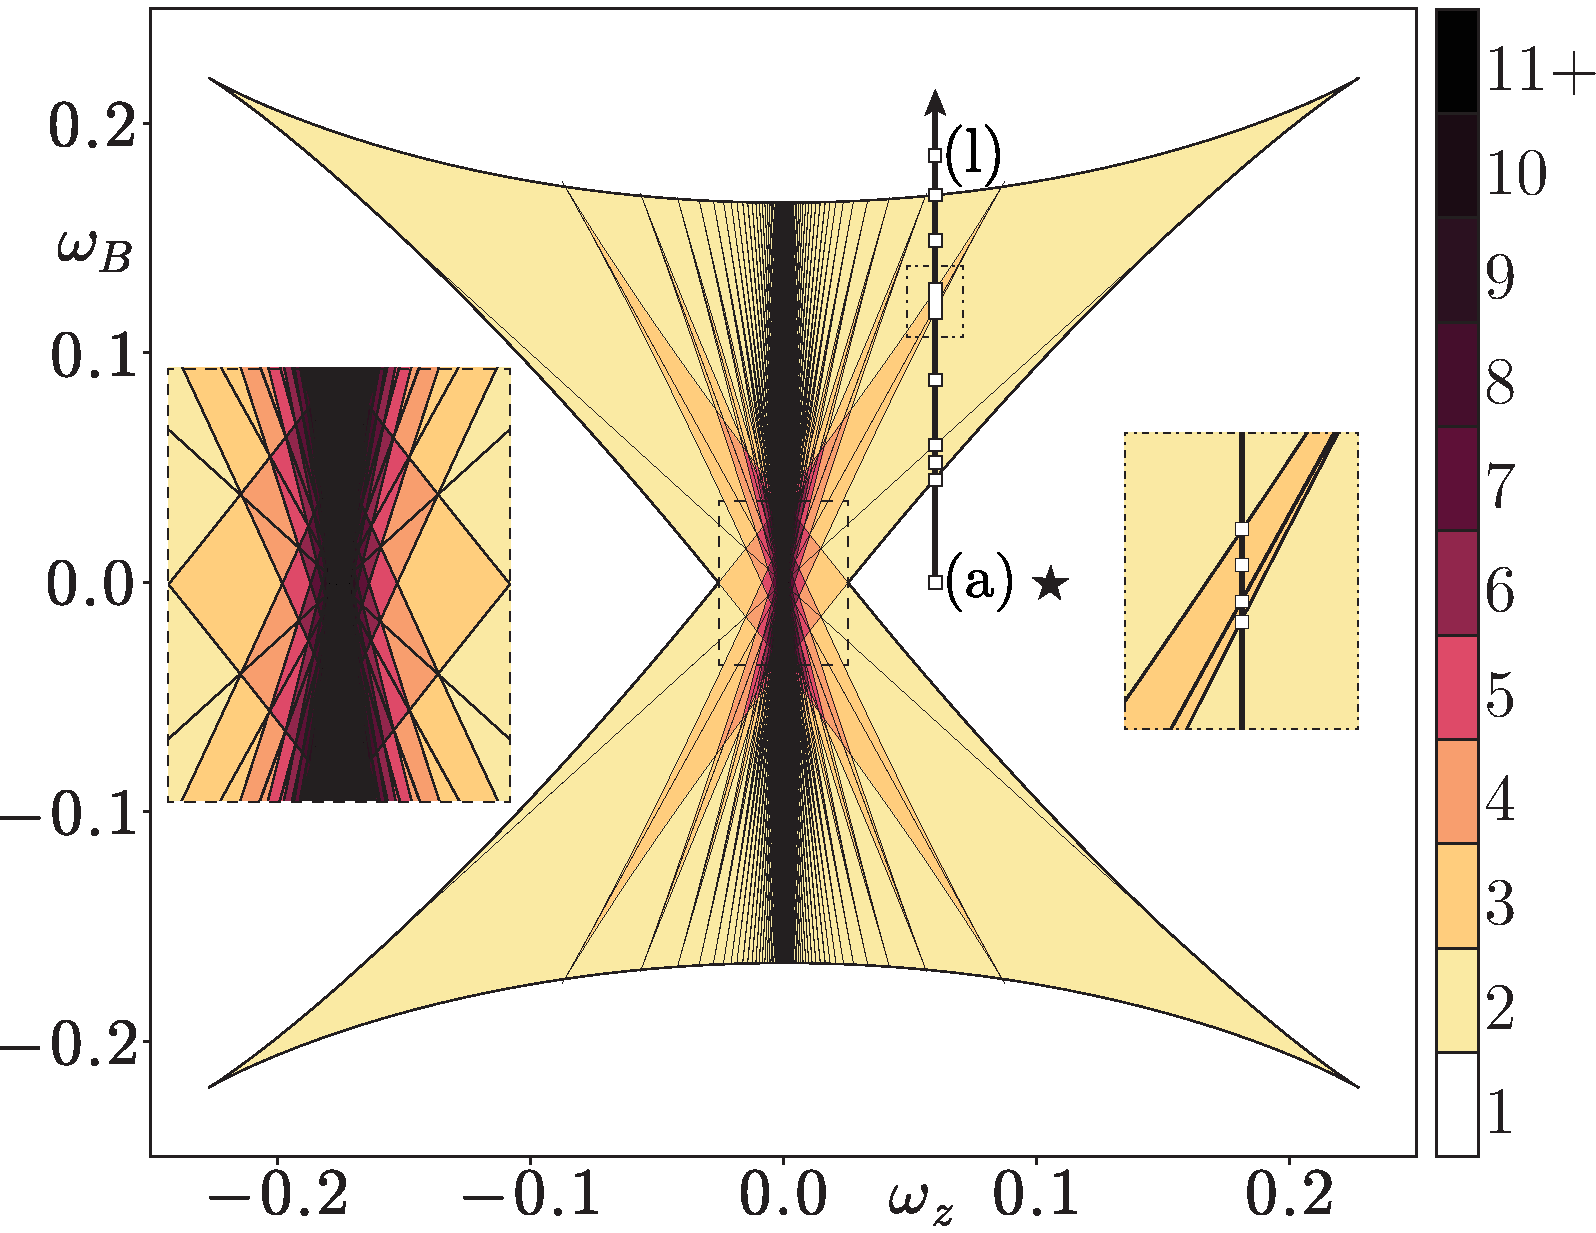
\includegraphics[width=\linewidth]{Images/EGM_components_2D_coloured_with_closeup.pdf}

    \caption{Regions in the $(\wz, \wB)$-plane indicating the number of isolated EGM-components exist up to 11 according to the colourbar. 
    A closeup of the region with the highest density of EGM components is shown in the inset.
    The values of $(\wz,\wB)$ plotted in Figure~\ref{fig:EGM_fold_varywB} are indicated by the dots along the line $\wz=0.06$.}

    \label{fig:EGM_components}
\end{figure}
%
\begin{figure}[!t]
    \centering
    \begin{overpic}[width=\linewidth]{Images/EGM_fold_varywB_wz006.pdf}
        % Row a
        \put(11.5,96){(a)}
        \put(36.5,96){(e)}
        \put(61.2,96){(i)}
        % Row b
        \put(11.5,72){(b)}
        \put(36.5,72){(f)}
        \put(61.2,72){(j)}
        % Row c
        \put(11.5,48){(c)}
        \put(36.5,48){(g)}
        \put(61.2,48){(k)}
        % Row d
        \put(11.5,24.5){(d)}
        \put(36.5,24.5){(h)}
        \put(61.2,24.5){(l)}
    \end{overpic}

    \caption{Graph of the EGM component function $G(\w_s)$ from \eqref{eq:EGM_components} for $\wz = 0.06$ and varying $\wB$, whose particular values are indicated by dots along the line $\wz=0.06$ in Figure~\ref{fig:EGM_components}.
    The roots (hollow circles) bound intervals of $\w_s$ values corresponding to egm components (thick lines); one interval always contains $\w_s = 0$ (the free running laser mode) and another contains the grating's Bragg frequency for $\wB \in [0.04505, 0.16895]$.
    }

    \label{fig:EGM_fold_varywB}
\end{figure}
%
The advantages of the discretised model in understanding the mode structure become apparent when examining the bifurcation patterns of the EGM solutions.
Analytic expressions for the EGM components and their bifurcation points can be derived from the discretised model, providing valuable insights into the stability and dynamics of the system.
The number of EGM components can be studied by setting the envelope of $f(\w_s)$ given by \eqref{eq:discretised_ws_envelope} equal to $g(\w_s)$, which yields the $\w_s$ values at the intersections as the roots of the function
%
\begin{equation}
    \label{eq:EGM_components}
    G(\w_s) = \w_s^2 - (1+\a^2)\left( \eta \, (1-t) \frac{S_N}{S} \right)^2.
 \end{equation}
 %
Moreover, these roots bound intervals of $\w_s$-values that correspond to different EGM-components, so that the function $G(\w_s)$ presents a geometrical interpretation of the EGM-components. 
The number of EGM-components changes when fold points (with respect to $\w_s$) of the envelope pass through the line $g(\w_s)$. 
These fold points are given by roots of the first derivative of \eqref{eq:EGM_components} with respect to $\w_s$, that is, by
%
\begin{gather}
    \label{eq:EGM_components_fold}
    \begin{aligned}
        \frac{\partial G}{\partial \w_s} &= \dt (1+\a^2)\left( \eta \, (1-t) \frac{S_N}{S} \right)^2 \times \\ 
        &\bigg(  \frac{t}{S^2} \sin(\phi_\text{F}) - N \frac{t^{N}}{{S_N}^2}\sin(N\phi_\text{F}) \bigg) + \w_s = 0.
    \end{aligned}
\end{gather}
%
\par
%
The locus of the passage through folds as the FBG parameters $\wz$ and $\wB$ are varied can be found with the pseudo-arclength continuation routines of \texttt{DDE-BifTool} \cite{sieber2014dde} to simultaneously solve the implicit equations \eqref{eq:EGM_components} and \eqref{eq:EGM_components_fold}, that is, by solving $G(\w_s) = \sfrac{dG}{d\w_s} = 0$.
Figure~\ref{fig:EGM_components} shows the locus of the passage through folds (computed by continuation) in projection onto the $(\w_s, \wB)$-plane.
In the white region outside the curve shown in Figure~\ref{fig:EGM_components} one finds a single EGM-component, while inside the shaded region there are two or more isolated EGM-components.
The outermost curves meet at cusp points.
Within this region containing more than one isolated component, further bifurcations can occur as $\wz$ and $\wB$ vary allowing for the emergence of an arbitrariry number of EGM components, as illustrated by the inset of Figure~\ref{fig:EGM_components}.
An explicit example of this behaviour can be seen in Figure~\ref{fig:EGM_fold_varywB}(a)-(l) which shows the the transition


the graph of $G(\w_s)$ for $\wz = 0.06$ and increasing $\wB \in [0, 0.018]$.
The number of EGM-components changes when fold points (with respect to $\w_s$) of the envelope pass through the line $G(\w_s) = 0$.
Finally, we note that the region shown in Figure~\ref{fig:EGM_components} scales linearly with the effective feedback strength $\eta (1-t) \sqrt{1 + \alpha^2}$.
In other words, the region retains its shape yet grows linearly with $\eta (1-t) \sqrt{1 + \alpha^2}$.
%
\par
%

%
\subsection{Stability Fluctuations}
\label{subsec:lichaos_skenderas}
%
\begin{figure}[t]
    
    \begin{overpic}[width=0.9\linewidth]{Images/Reflection_zero_overlap.pdf}
        \put(2,86){(a)}
        \put(2,43){(b)}
    \end{overpic}

    \caption{Caption}
    
    \label{fig:zero_overlap}
\end{figure}
%
It is important to note that while the locations of zeros in the discretised model are uniform, is only the case for FBGs which have relatively low reflectivities, see Figure~\ref{fig:uniform_spectra_varykL}. 
For this, re 
%

\begin{figure}[t]
    \flushleft
    \begin{overpic}[width=0.845\linewidth]{Images/Li_chaos_heatmap_image.pdf}
        \put(-2,77){(a)}
    \end{overpic}\\
    \vspace{-0.5em}
    \begin{overpic}[width=0.99\linewidth]{Images/discretised_Lichoatic_wBeta_comparison_hopfs_minbifs_ai.pdf}
        \put(-2,65){(b)}
    \end{overpic}\\
    \vspace{-0.5em}
    \begin{overpic}[width=\linewidth]{Images/discretised_Lichoatic_wBeta_comparison_lyapunovs.pdf}
        \put(-2,70){(c)}
    \end{overpic}

    \caption{Comparison between two parameter dynamical mappings of output intensity for a convolved FBG feedback form of $F(t)$ \cite{li2012distributed,li2015chaotic,li2020stable} (a) 
    and the discretised FBG feedback form of $F(t)$ in the parameter space of feedback strength ($\xi_f$ in (a) and equivalent $\eta$ in (b)) 
    and grating detuning frequency ($\Delta f$). 
    In (a), the laser output intensity is stable (white), period-one oscillatory (red), quasi-periodic pulsating (gray), period-doubled oscillatory (yellow), and chaotic (black). 
    In (b), the laser output is in steady-state (white), period-one oscillatory (red), period-two (yellow), and period 3 to very large period in a gradient from grey to black. 
    In (c) parameter sweeps are performed in all four directions, with Hopf bifurcations of steady state EGMs overlayed.}
    
    \label{fig:Li_chaos}
\end{figure}
%
\par
%
Finally, we compare our model to the most recent work on semiconductor lasers under FBG feedback by \Skenderas \textit{ et al.} \cite{skenderas2021feedback,skenderas2024impact}. 
In contrast to the previous two models, where nondimensionalisations and approximations were required before direct comparisons could be made, the form of the equations analysed mirror the equations presented in this work, 
using parameter values $(\a, P, T, \tau) = (3, 1, 1000, 1000)$, except for the use of a convolution feedback term $F(t)$ of the form \eqref{eq:convolution}. 
The results presented by \Skenderas \textit{ et al.} therefore serve as the most suitable basis for comparisons in the accuracy of the derived discretised model. 
Given the complexity of analysing the LK equations under FBG feedback using a convolution term, the results presented, 
like those previously studied, are obtained solely through analysis of time series obtained through numerical integration. 
The main focus of their analysis is in characterising the interplay between the lasers relaxation oscillations (ROs) and the FBG reflection zeros as a function of feedback rate $\eta$ and grating bandwidth $\wz$ for varying feedback phase $C_p$ and grating detuning $\omega_B$. 
%
\par
%
ROs are the most typical type of oscillation that one would expect in semiconductor lasers. 
They are damped intensity fluctuations that occur when the laser transitions between steady states, typically after a sudden change in injection current, 
and arise from the dynamic interplay between photon density and carrier density in the laser cavity. 
When the carrier population is perturbed, it overshoots the steady-state value, causing oscillations in output power at a characteristic frequency known as the relaxation oscillation frequency $\w_\text{RO}=\sqrt{2P/T}$, 
which form the dominant side lobes either side of the centre frequency in the Fourier spectrum of a semiconductor laser. 
Exciting the ROs of a laser can lead to a more unstable laser, and therefore one would expect that lower amount of feedback would cause the laser to transition from steady output to oscillatory and then more unstable outputs. 
%
\par
%
The strategy employed by the authors to observe this behaviour is by tracking the Hopf bifurcation of the steady state of the laser in the $(L_\text{FBG},\eta)$-plane, 
where the grating length $L_\text{FBG}$ can be used to control the grating bandwidth $\wz$ as discussed in \ref{sec:EGM_discretised}. 
As discussed in \ref{sec:FBG}, varying the grating length also changes the grating reflectivity, therefore, when using this model, grating parameters must be simultaneously varied to solely vary its bandwidth. 
This is not an issue with the discretised reflections model as bandwidth $\wz$ and thus length $L_\text{FBG}$ can be varied independent of reflectivity using \ref{eq:wz_approx}
%
\begin{equation}
    L [\text{m}] \approx \frac{\pi c \tau_p}{\wz \neff} 
\end{equation}
%
where $\tau_p$ is the photon lifetime used to rescale time in this form of the LK equations as discussed in Section~\ref{sec:EGM_discretised}.
%
\par
%
\begin{figure}[!t]
    \flushright
    \begin{overpic}[width=\linewidth]{Images/discretised_Skenderas_wzeta_Cpcomparison_N20.pdf}
        \put(-3,55){(a)}
    \end{overpic}\\
    \hspace{-0.5em}
    \begin{overpic}[width=0.98\linewidth]{Images/discretised_Skenderas_wBeta_image.pdf}
        \put(-3,75){(b)}
    \end{overpic}\\
    \hspace{-0.5em}
    \begin{overpic}[width=0.97\linewidth]{Images/discretised_Skenderas_wBeta_comparison_minbifs_ai.pdf}
        \put(-3,75){(c)}
    \end{overpic}

    \caption{The evolution of Hopf bifurcation tracking the stability fluctuations as a function of $L_\text{FBG}$ at zero detuning for different values of the feedback offset phase $C_p$ equal to 
    $0$ (blue), $\pi /4$ (yellow), $\pi/2$ (violet), $2\pi/3$ (green), $\pi$ (cyan), $3\pi/2$ (maroon), and $7\pi/4$ (orange). Comparison between two parameter dynamical mappings of output intensity for a convolved FBG feedback form of $F(t)$ \cite{li2012distributed,li2015chaotic,li2020stable} (a) 
    and the discretised FBG feedback form of $F(t)$ in the parameter space of feedback strength ($\xi_f$ in (a) and equivalent $\eta$ in (b)) and grating detuning frequency ($\Delta f$). 
    In (a), the laser output intensity is stable (white), period-one oscillatory (red), quasi-periodic pulsating (gray), period-doubled oscillatory (yellow), and chaotic (black). 
    In (b), the laser output is in steady-state (white), period-one oscillatory (red), period-two (yellow), and period 3 to very large period in a gradient from grey to black. 
    In (c) parameter sweeps are performed in all four directions, with Hopf bifurcations of steady state EGMs overlayed}
    
    \label{fig:Skenderas_wBeta}
\end{figure}
%


% !TeX root = ../main.tex
\section*{Conclusions and future developments}
\label{sec:conclusions}
%
While a low reflectivity $R$ does provide the desired transmission zeros, the relative errors in both total reflectivity $R_\text{error}$ and delay $\tau_\text{error}$ are larger compared to larger total reflectivities. 
This is demonstrated in Figure~\ref{fig:NR_Selection}, which visualises the combined relative errors $R_\text{error}$ and $\tau_\text{error}$ using the Euclidean metric $\| R_\text{error}, \tau_\text{error} \|_{_2} = \sqrt{R_\text{error}^2 + \tau_\text{error}^2}$. 
For the choice $N=10$, a total reflectivity $R_\text{approx} = 0.75$ would provide a lower combined error of 4\% as shown in (a) compared to the $R_\text{approx} = 0.1$ which has a combined error of 19\%. 
As the ability to effectively describe and analyse transmission zeros of FBGs is of great interest, this increase in combined error, which is still relatively low from a modelling perspective, is a an acceptable trade-off.
%
\begin{figure}
    \centering
    
    \includegraphics[width=0.95\linewidth]{Images/NR_Selection.pdf}
    
    \caption{Combined relative errors of FBG total reflectivity $R_\text{error}$ and delay $\tau_\text{error}$ as a function of the grating number $N$ and normalised refractive index variation $\dn$. 
    Level sets of constant total reflectivity $R_\text{approx}$ are overlayed in white. 
    In (a), the square marker at $(N,\dn) = (10, 0.07)$, corresponding to an $R_\text{approx} = 0.75$ has a combined error of 4\% while in (b), the marker at $(N,\dn) = (10, 0.0055)$, 
    corresponding to an $R_\text{approx} = 0.1$ has a combined error of 19\%.}
    
    \label{fig:NR_Selection}
\end{figure}
%

% =======================
% Acknowledgments (optional)
% =======================
\begin{acknowledgments}
We acknowledge ...
\end{acknowledgments}

% =======================
% Appendices (optional, modular)
% =======================
\appendix
% !TeX root = ../main.tex
\section{Nondimensionalisation of the original LK Equations}
\label{app:LK_nondim}
%
\let\cleardoublepage\origcleardoublepage
%
The LK equations in dimensional form are
%
\begin{gather}
\label{eq:dimensionalised_LK}
\begin{aligned}
\frac{d E}{d s} &= \tfrac{1}{2} G_{\mathrm{M}0}(1 + i \alpha)\,(N - N_N) E 
+ \kappa_0 e^{-i C_p} F(s, \tau_0), \\[0.3em]
\frac{d N}{d s} &= J_0 - \gamma_0 N 
- \left[\Gamma_{\mathrm{M}0} + G_{\mathrm{N}0}(N - N_N)\right] |E|^2,
\end{aligned}
\end{gather}
%
where \(E\) is the slowly varying complex field amplitude and \(N\) the carrier density.
The parameters are defined as follows: 
\(\alpha\) is the linewidth enhancement factor, 
\(\gamma_0\) the carrier decay rate, 
\(\Gamma_{\mathrm{M}0}\) the cavity decay rate, 
\(\kappa_0\) the feedback strength, 
and \(\tau_0\) the external round–trip delay. 
The material response enters through the small-signal gain coefficients 
\(G_{\mathrm{M}0}\) and \(G_{\mathrm{N}0}\), 
while \(J_0\) denotes the pump current and \(N_N\) the inversion at threshold.
%
\par
%
To simplify the equations and reduce the number of parameters, we introduce scaled variables
\[
X = \frac{G_{\mathrm{M}0}}{2 \gamma_p}(N - N_N), 
\qquad 
A = \sqrt{\frac{G_{\mathrm{N}0}}{2 \gamma_0}}\, E,
\]
where \( \gamma_p = \Gamma_{\mathrm{M}0} G_{\mathrm{M}0} / G_{\mathrm{N}0} \) is a rescaled photon lifetime. 
Rescaling time as \( t = \gamma_p s \), the Lang–Kobayashi equations become
\[
\begin{gathered}
\frac{d A}{d t} = (1 + i \alpha)\, A X + \eta e^{-i C_p} F(t,\tau), \\[0.3em]
T \frac{d X}{d t} = P - X - (1 + 2X)|A|^2.
\end{gathered}
\]
Here, the dimensionless parameters are defined as follows. 
The pumping rate above threshold is 
\[
P = \frac{G_{\mathrm{M}0}}{2 \gamma_p \gamma_0}(J_0 - \gamma_0 N_N),
\]
the ratio of photon to carrier lifetime is 
\[
T = \frac{\gamma_p}{\gamma_0},
\]
the normalized feedback strength is 
\[
\eta = \frac{\kappa_0 G_{\mathrm{N}0}}{G_{\mathrm{M}0} \Gamma_{\mathrm{M}0}},
\]
and the rescaled external delay is 
\[
\tau = \gamma_p \tau_0.
\]
%
As a concrete example, consider the dimensionalised parameters  
$
\alpha = 3.5, \; 
\gamma_0 = 1.0 \times 10^9, \; 
\Gamma_{\mathrm{M}0} = 0.55 \times 10^9, \;
\kappa_0 = 25.0 \times 10^9, \; 
\tau_0 = 0.22 \times 10^{-9}, \;
G_{\mathrm{M}0} = 50.0, \; 
G_{\mathrm{N}0} = 0.05, \; 
J_0 = 8.0 \times 10^9, \; 
N_N = 5.0.
$
%
These yield a rescaled photon lifetime \(\gamma_p = 5.5 \times 10^{11}\), giving the nondimensionalised parameters
%
$
\alpha = 3.5, \; 
P = 0.136, \; 
T = 550, \; 
\eta = 0.0455, \; 
\tau = 121,
$
%
which are the values used in Sections~\ref{subsec:FBG_discretised_derivation} and~\ref{subsec:EGM_structure}.  
%
\par
%
The nondimensionalised time unit corresponds to a photon lifetime of \(\tau_p = 1/\gamma_p = 1.82 \times 10^{-12}\,\text{s}\). 
For operation at \(\lambda = 1550\,\text{nm}\), the laser angular frequency is \(\omega_c = 1216\,\text{rad\,ps}^{-1}\). 
It follows that \(\wz\) in the LK equations is dimensionless, normalised by \(\tau_p = 1/\gamma_p = 1.82\,\text{ps}\). 
With this scaling, the angular frequency is nondimensionalised to \(\omega_{\max} = 2211\), which in turn requires \(N \approx 22{,}500\) layers according to~\eqref{eq:wz_approx}.
%
%
\subsection{Discretisation of dimensionalised convolution FBG–LK model}
\label{app:Li_chaos_nondim}
%
We show here how the convolution-based model of Li \textit{et al.} \cite{li2012distributed,li2015chaotic,li2020stable} reduces, under mild and explicitly stated approximations, to the dimensionalised LK form \eqref{eq:dimensionalised_LK} used throughout this paper.
%
Li \textit{et al.} consider
%
\begin{equation} 
    \left\{ 
        \begin{aligned} \frac{d a}{d t} &= \frac{1-i b}{2} \left[\frac{\gamma_{c} \gamma_{n}}{\gamma_{s} \tilde{J}} \tilde{n} - \gamma_{p}\left(|a|^{2}-1\right)\right] a \\ 
            &\hspace{2cm} + \gamma_{c} \xi_{f} e^{i \theta} \left[r(t) e^{-i \Delta \Omega t}\right] * a\!\left(t-\tau_\text{RT}\right) \\ 
            \frac{d \tilde{n}}{d t} &= -\left(\gamma_{s}+\gamma_{n}|a|^{2}\right) \tilde{n} - \gamma_{s} \tilde{J}\left(1-\frac{\gamma_{p}}{\gamma_{c}}|a|^{2}\right) \left(|a|^{2}-1\right) 
        \end{aligned} \right. 
\end{equation}
%
where $r(t)$ is the impulse response associated with the FBG reflectivity and $\Delta\Omega$ is the grating detuning. 
For consistency with \eqref{eq:dimensionalised_LK}, define the notational relabeling
$
a=E,\; \tilde{n}=N,\;
F(t):=\big[r(t)e^{-i\Delta\Omega t}\big]*E\!\left(t-\tau_{\rm RT}\right),\; t=s,
$
 which gives
\begin{equation}
\label{eq:Li_rewritten}
\left\{
\begin{aligned}
\frac{d E}{d s} &= \frac{1-ib}{2}
\left[\frac{\gamma_{c}\gamma_{n}}{\gamma_{s}\tilde{J}}\,N
      -\gamma_{p}\big(|E|^{2}-1\big)\right]E
+ \gamma_{c}\,\xi_{f}\, e^{i\theta} F, \\
\frac{d N}{d s} &= -\big(\gamma_{s}+\gamma_{n}|E|^{2}\big) N
   - \gamma_{s}\tilde{J}\!\left(1-\frac{\gamma_{p}}{\gamma_{c}}|E|^{2}\right)\!\big(|E|^{2}-1\big).
\end{aligned}
\right.
\end{equation}
%
\par
%
We assume the usual near-threshold/weak-saturation ordering used by Li \textit{et al.}:
%
\[
\frac{\gamma_{c}\gamma_{n}}{\gamma_{s}\tilde{J}} \gg \gamma_{p},
\]
so the $-\tfrac{1-ib}{2}\gamma_p(|E|^2-1)E$ term may be dropped in the field equation to leading order. 
Under this ordering, \eqref{eq:Li_rewritten} becomes
\begin{equation}
\label{eq:Li_leading}
\left\{
\begin{aligned}
\frac{d E}{d s} &\approx 
\frac{1}{2}\frac{\gamma_{c}\gamma_{n}}{\gamma_{s}\tilde{J}}\,(1-ib)\,N E
+ \gamma_{c}\xi_f e^{i\theta} F,\\[0.25em]
\frac{d N}{d s} &= -\gamma_s N - \gamma_n|E|^2 N 
- \gamma_s\tilde{J}\!\left(1-\frac{\gamma_p}{\gamma_c}|E|^2\right)\!(|E|^2-1).
\end{aligned}
\right.
\end{equation}
Expanding the carrier equation and grouping powers of $|E|^2$ yields
\begin{align*}
\frac{d N}{d s} 
&= \gamma_s\tilde{J} - \gamma_s N 
  - \Big[\gamma_s\tilde{J}\!\left(1+\tfrac{\gamma_p}{\gamma_c}\right)+\gamma_n N\Big]|E|^2
  + \frac{\gamma_s\gamma_p\tilde{J}}{\gamma_c}|E|^4.
\end{align*}
Neglecting the quartic term $|E|^4$ under weak saturation gives the closed system
\begin{equation}
\label{eq:Li_reduced}
\left\{
\begin{aligned}
\frac{d E}{d s} &= 
\frac{1}{2}\frac{\gamma_{c}\gamma_{n}}{\gamma_{s}\tilde{J}}\,(1-ib)\,N E
+ \gamma_{c}\xi_f e^{i\theta} F,\\
\frac{d N}{d s} &= \gamma_s\tilde{J} - \gamma_s N 
- \Big[\gamma_s\tilde{J}\!\left(1+\tfrac{\gamma_p}{\gamma_c}\right)+\gamma_n N\Big]|E|^2.
\end{aligned}
\right.
\end{equation}
%
\par
%
Comparing \eqref{eq:Li_reduced} with \eqref{eq:dimensionalised_LK}, we obtain the one-to-one parameter correspondence
%
$
b=-\alpha,\; \theta=-C_p,\; 
G_{\mathrm{M}0}=\gamma_c\gamma_n/\gamma_s\tilde{J},\;
\kappa_0=\gamma_c\xi_f,\;
J_0=\gamma_s\tilde{J},\; 
\gamma_0=\gamma_s,\; 
\Gamma_{\mathrm{M}0}=\gamma_s\tilde{J}\!\left(1+\gamma_p/\gamma_c\right),\;
G_{\mathrm{N}0}=\gamma_n,
$
%
and the external delay $\tau_0=\tau_{\rm RT}$. 
The convolution kernel $r(t)e^{-i\Delta\Omega t}$ plays the role of the (dimensioned) impulse response used in \eqref{eq:dimensionalised_LK}, with $\Delta\Omega$ corresponding to the grating detuning.
%
\par
%
In summary, under the standard weak-saturation ordering and after neglecting the quartic $|E|^4$ term, the convolution-based equations of \cite{li2012distributed,li2015chaotic,li2020stable} reduce exactly to the dimensionalised LK form \eqref{eq:dimensionalised_LK}, with the above parameter identifications and with the feedback written as a time-domain convolution against the FBG impulse response.
This establishes the formal equivalence used for the comparisons in the main text.
%
%
\section{Discretisation of multiple external-cavity reflections in the FBG LK model}
\label{app:EC_multiple}
%
A key extension of the single-reflection Lang–Kobayashi model is to include multiple reflections within the EC. 
In this case, the reflected field can be written as
\begin{equation*}
    E_r(t) = E(t) + \frac{R_2^2 - 1}{R_2^2} \sum_{n=1}^\infty (-R_2 R)^n e^{-i n C_p} E(t-n \tau),
\end{equation*}
%
where $R_2$ is the reflectivity of the front facet of the laser, $R$ the external mirror reflectivity, and $C_p$ the cavity phase. 
Truncating this series to first order recovers the familiar single-reflection feedback term. 
Indeed, expanding the logarithm in the feedback term gives
%
\begin{equation*}
    \begin{aligned}
    E(t) \ln{\!\left(\frac{E_r(t)}{E(t)}\right)} 
    &\approx E(t)\!\left(\frac{\tfrac{R_2^2 - 1}{R_2^2}(-R_2 R)e^{-i C_p} E(t-\tau)}{E(t)}\right) \\
    &= \eta e^{-i C_p} E(t-\tau),
    \end{aligned}
\end{equation*}
%
as expected.
%
%
\subsubsection*{Multiple-reflection formulation}
%
Naumenko \textit{et al.} \cite{naumenko2003characteristics,naumenko2004slow} generalised the LK equations to explicitly incorporate this logarithmic multiple-reflection term:
%
\begin{equation*} 
    \left\{\begin{aligned}
         \frac{d E}{d s} &= \frac{1}{2} \tau_\text{in} \Gamma G_N(1+i \alpha)\left(N-N_{\text {th }}\right) E + \ln \left(\frac{\bar{F}}{E}\right) E \\ 
        \frac{d N}{d s} &= \frac{\tau_{\text{in}}\left(J-\bar{J}_0\right)}{e V}-\frac{\tau_\text{in}}{\tau_e} N-\left[\frac{\tau_\text{in}}{\Gamma \tau_{ph}}+G_N \tau_\text{in}\left(N-N_{\text{th}}\right)\right]|E|^2 
    \end{aligned}\right. 
\end{equation*}
%
with
%
\begin{gather} 
    \begin{aligned} 
    \bar{F}(t) &= E+\frac{(-1)}{2 \pi} \frac{\left(1-r_2^2\right)}{r_2^2} \sum_{n=1}^{\infty} e^{-i \omega_0 n \tau} \times \\ 
    &\int_{-\infty}^{+\infty} d \omega\left(-r_2 r_B(\omega)\right)^n e^{i \omega(t-n \tau)} \int_{-\infty}^{+\infty} d t^{\prime} E\left(t^{\prime}\right) e^{-i \omega t^{\prime}} 
    \end{aligned} 
\end{gather}
%
%
\subsubsection*{Reduction to the standard LK form}
%
By neglecting gain compression ($\epsilon \approx 0$) and thermal detuning ($k=0$), and linearising the spontaneous emission term, the equations reduce to
%
\begin{equation*}
\left\{
\begin{aligned}
\frac{d E}{d t} &= \tfrac{1}{2} \Gamma G_N(1+i \alpha)(N-N_\text{th}) E 
+ \frac{1}{\tau_\text{in}} \ln \!\left(\tfrac{\bar{F}(t)}{E}\right) E, \\
\frac{d N}{d t} &= \frac{J-\bar{J}_0}{e V}-\frac{N}{\tau_0}
-\Big[\tfrac{1}{\Gamma \tau_{ph}} + G_N(N-N_\text{th})\Big]|E|^2.
\end{aligned}
\right.
\end{equation*}
%
Rescaling time by $t=\tau_\text{in} s$ yields
%
\begin{equation*}
\left\{
\begin{aligned}
\frac{d E}{d s} &= \tfrac{1}{2} \tau_\text{in} \Gamma G_N(1+i \alpha)(N-N_{\text{th}}) E + \ln \!\left(\tfrac{\bar{F}}{E}\right) E, \\
\frac{d N}{d s} &= \tfrac{\tau_{\text{in}}(J-\bar{J}_0)}{e V}-\tfrac{\tau_\text{in}}{\tau_e} N
-\Big[\tfrac{\tau_\text{in}}{\Gamma \tau_{ph}}+G_N \tau_\text{in}(N-N_{\text{th}})\Big]|E|^2,
\end{aligned}
\right.
\end{equation*}
%
which matches the dimensionalised LK form \eqref{eq:dimensionalised_LK} when identifying
%
$
\alpha = \alpha, \; 
N_N = N_{\text{th}}, \; 
G_\text{M0} = \tau_\text{in} \Gamma G_N, \; 
G_\text{N0} = G_N \tau_\text{in}, \;
J_0 = \tau_\text{in}(J-\bar{J}_0)/e V, \;
\gamma_0 = \tau_\text{in}/\tau_e, \; 
\Gamma_\text{M0} = \tau_\text{in}/\Gamma \tau_{ph}, \; 
\tau_0 = 2 L_\text{ext} n_\text{ext}/c \tau_\text{in}
$.
%
\par
%
Finally, the multiple-reflection feedback term reduces in the single-reflection limit to
%
\begin{equation*}
    E \ln \left(\tfrac{\bar{F}}{E}\right) \approx \frac{1-R_2^2}{R_2} e^{-i C_p} F,
\end{equation*}
%
so that
%
\begin{equation*}
    \kappa_0 = \frac{1-R_2^2}{R_2} R.
\end{equation*}
%
\par
%
Thus the Naumenko model and the standard LK formulation are equivalent up to the choice of effective feedback strength, completing the connection between multiple- and single-reflection descriptions.
%
%
subsection{Derivation of Variational equations for the Discretised reflection FBG LK Equations}
\label{app:lyapunov}
%
Beginning with the discretised reflections model, consisting of the complex valued electric field variable $E$ and real valued carrier density variable $N$ \eqref{eq:LK_discretised}, the variational equations are defined as
%
\begin{equation}
    \frac{d}{d t}\binom{\delta E}{\delta N} = \mathbf{J}(\underline{F})\binom{\delta E}{\delta N} + \sum_{k=1}^{N}\mathbf{J}_{\tau_{k}}(\underline{F})\binom{\delta E_{\tau_{k}}}{\delta N_{\tau_{k}}}
\end{equation}
%
where $\underline{F}(t)=(\dot{E}(t), \dot{N}(t))^T$, which results in
%
\begin{gather}
\begin{aligned}
    \label{eq:variational}
    \dot{\delta E}(t) &= (1+i \alpha)[\delta E \; N + E \; \delta N]\\
                &\hspace{1cm} + \eta(1-t) e^{-i C_p} \sum_{k=0}^{N-1} t^{k} e^{-i \wB \dt} \delta E\left(t-\tau_{k}\right) \\
    \dot{\delta N}(t) &=-\frac{1}{T}\left[2(1+2 N) \text{Re}\left\{\overline{E} \; \delta E\right\} + (1+2|E|^{2} ) \delta N \right].
\end{aligned}
\end{gather}
%
These variational equations then can be used to calculate Lyapunov spectra as done in this work using the method outlined in \cite{farmer1982chaotic}.


% =======================
% Bibliography
% =======================
\bibliographystyle{apsrev4-2}
\bibliography{bibliography}
% =======================

\end{document}
